% !TeX program = pdflatex
% Composition root (controller): document order belongs here.
\documentclass[11pt,letterpaper]{article}

% !TeX root = ../../main.tex
% Package dependencies (view infrastructure).
\usepackage[T1]{fontenc}
\usepackage[utf8]{inputenc}
\usepackage{lmodern}
\usepackage[margin=0.82in,headheight=15pt]{geometry}
\usepackage[nopatch=footnote]{microtype}
\usepackage{amsmath,amssymb,mathtools,bm}
% Load array before longtable/tabularx so their internal column hooks agree
% across MiKTeX package versions.
\usepackage{array}
\usepackage{booktabs,longtable,tabularx,multirow}
% No table-cell coloring is used; omitting the table option also avoids
% coupling colortbl internals to a particular array package release.
\usepackage[dvipsnames]{xcolor}
\usepackage{enumitem}
\usepackage{graphicx}
\usepackage{tikz}
\usetikzlibrary{arrows.meta,positioning,fit,shapes.geometric,calc}
\usepackage[most]{tcolorbox}
\usepackage{fancyhdr}
\usepackage{titlesec}
\usepackage{natbib}
\usepackage[hidelinks]{hyperref}
\usepackage{xurl}
\usepackage[nameinlink,noabbrev]{cleveref}
\usepackage{url}
\usepackage{setspace}
\usepackage{caption}
\usepackage{tocloft}

% !TeX root = ../../main.tex
% Single source of truth for document metadata (model).
\newcommand{\PaperTitle}{Where the Quantum Work Actually Is}
\newcommand{\PaperSubtitle}{Engineering Effective Algorithms Under Physical Bounds}
\newcommand{\PaperTagline}{A problem-first framework from phase encodings to particle physics and astronomy}
\newcommand{\PaperAuthor}{Vi Connelly}
\newcommand{\PaperAffiliation}{Independent Researcher and Software Engineer}
\newcommand{\PaperDate}{August 2026}
\newcommand{\PaperRunningTitle}{Quantum Algorithm Engineering Under Physical Bounds}
\newcommand{\PaperSubject}{A problem-first framework for engineering quantum and hybrid algorithms}
\newcommand{\PaperPdfKeywords}{quantum algorithms, resource estimation, hybrid computing, quantum error correction, particle physics, astronomy}
\newcommand{\PaperKeywords}{quantum algorithms; resource estimation; hybrid quantum-classical computing; quantum error correction; quantum simulation; high-energy physics; astronomy; scientific computing}
\newcommand{\PaperCentralClaim}{A problem becomes a credible quantum candidate only when its expensive classical bottleneck can be expressed as an efficiently implementable coherent transformation, a useful global property can be extracted through interference, and the complete workflow survives the costs of preparation, routing, error control, measurement, verification, and classical competition.}

% !TeX root = ../../main.tex
% Shared semantic commands. Add notation here instead of redefining it in sections.
\newcommand{\E}{\mathbb{E}}
\newcommand{\Var}{\operatorname{Var}}
\newcommand{\TTS}{\operatorname{TTS}}
\newcommand{\ket}[1]{\left|#1\right\rangle}
\newcommand{\bra}[1]{\left\langle#1\right|}
\newcommand{\braket}[2]{\left\langle#1\middle|#2\right\rangle}
\newcommand{\norm}[1]{\left\lVert#1\right\rVert}

% !TeX root = ../../main.tex
% Visual system (view): color, spacing, page furniture, headings, and callouts.
\setlength{\cftbeforesecskip}{0.35em}
\setlength{\cftbeforesubsecskip}{0pt}

\definecolor{ink}{HTML}{18232B}
\definecolor{quantum}{HTML}{0B6E75}
\definecolor{quantumdark}{HTML}{084B50}
\definecolor{mist}{HTML}{EAF5F4}
\definecolor{warm}{HTML}{F5EEE6}
\definecolor{warning}{HTML}{9C3D2E}
\definecolor{softgray}{HTML}{F4F6F7}

\hypersetup{
  pdftitle={\PaperTitle: \PaperSubtitle},
  pdfauthor={\PaperAuthor},
  pdfsubject={\PaperSubject},
  pdfkeywords={\PaperPdfKeywords},
  colorlinks=true,
  linkcolor=quantumdark,
  citecolor=quantumdark,
  urlcolor=quantum
}

\pagestyle{fancy}
\fancyhf{}
\fancyhead[L]{\small\textcolor{quantumdark}{\PaperRunningTitle}}
\fancyhead[R]{\small\textcolor{ink}{\PaperAuthor}}
\fancyfoot[C]{\small\thepage}
\renewcommand{\headrulewidth}{0.35pt}

\titleformat{\part}[block]
  {\centering\LARGE\bfseries\color{quantumdark}}
  {Part \thepart}{0.65em}{}
\titleformat{\section}{\Large\bfseries\color{quantumdark}}{\thesection}{0.65em}{}
\titleformat{\subsection}{\large\bfseries\color{ink}}{\thesubsection}{0.55em}{}
\titleformat{\subsubsection}{\normalsize\bfseries\color{quantumdark}}{\thesubsubsection}{0.5em}{}
\titlespacing*{\part}{0pt}{2.6ex plus 0.6ex}{1.5ex}
\titlespacing*{\section}{0pt}{2.1ex plus 0.5ex}{0.8ex}
\titlespacing*{\subsection}{0pt}{1.7ex plus 0.4ex}{0.5ex}

\setlist[itemize]{leftmargin=1.35em,itemsep=0.35em,topsep=0.35em}
\setlist[enumerate]{leftmargin=1.55em,itemsep=0.45em,topsep=0.35em}
\renewcommand{\arraystretch}{1.16}
\captionsetup{font=small,labelfont=bf}
\setlength{\parindent}{1.15em}
\setlength{\parskip}{0.15em}
\setlength{\emergencystretch}{2em}

\newtcolorbox{thesisbox}[1][]{
  enhanced,
  breakable,
  colback=mist,
  colframe=quantum,
  boxrule=0.7pt,
  arc=1.2mm,
  left=2.2mm,right=2.2mm,top=1.6mm,bottom=1.6mm,
  fonttitle=\bfseries,
  title=#1
}

% Decorative page-border system (self-contained; disable with \floralbordersfalse).
% !TeX root = ../../main.tex
% ---------------------------------------------------------------------------
% Deterministic geometric violet floral page borders (presentation layer).
%
% Design contract:
%   * Vector-only TikZ ornament drawn on a shipout background layer (eso-pic),
%     so it never affects bounding boxes, line breaking, or pagination.
%   * All ornament is hard-clipped to two vertical margin bands, one along
%     each page edge: x in [FloralBandMin, FloralBandMax] mm from the edge,
%     y in [FloralBandVPad, paperheight-FloralBandVPad] mm.  With letterpaper
%     and 0.82in (20.8mm) text margins this leaves >= 6.8mm of empty space
%     between any ornament and the content rectangle, keeps the running
%     header (which starts 20.8mm from the left edge) untouched, and leaves
%     the bottom-center page-number zone completely empty.
%   * Determinism: page_seed = FloralBaseSeed + FloralSeedPrime * abspage,
%     where abspage is a private absolute shipout counter (independent of
%     roman/arabic numbering).  The PGF random seed is reset from this value
%     at the start of every physical page, so no page's art depends on
%     earlier drawing.  BASE = 104729, PRIME = 9973 (both fixed; documented
%     here as required).  Randomness selects only among prevalidated slots
%     and bounded parameter ranges -- never free coordinates.
%   * Disable everything with \floralbordersfalse (before \begin{document}).
% ---------------------------------------------------------------------------

\newif\iffloralborders
\floralborderstrue
\makeatletter

% --- fixed seeds (see header comment) --------------------------------------
\def\FloralBaseSeed{104729}
\def\FloralSeedPrime{9973}

% --- master knobs -----------------------------------------------------------
\def\FloralOpacityScale{1.0}   % master opacity multiplier
\def\FloralFrameX{7.0}         % frame-line inset from page edge (mm)
\def\FloralBandMin{2.0}        % clip band, min distance from edge (mm)
\def\FloralBandMax{14.0}       % clip band, max distance from edge (mm)
\def\FloralBandVPad{7.0}       % clip band, vertical padding top/bottom (mm)
\def\FloralMotifX{9.4}         % nominal motif-center distance from edge (mm)

% --- palette (defined once; violet family + one restrained gold accent) -----
\definecolor{floralDeep}{HTML}{4A2E63}   % deep violet/plum: outlines, centers
\definecolor{floralMid}{HTML}{7C4E9F}    % medium violet: primary petals
\definecolor{floralLav}{HTML}{A88FC7}    % muted lavender: secondary petals
\definecolor{floralLilac}{HTML}{D9CBE9}  % pale lilac: low-opacity accents
\definecolor{floralGold}{HTML}{A9853B}   % rare complementary accent

% --- absolute page counter ---------------------------------------------------
\newcount\floral@abspage
\newcount\floral@seed
\newcount\floral@seedtmp

% --- bounded random helpers (pgf stream, reseeded per page) ------------------
% \floral@rnd{\macro}{min}{max} -> integer in [min,max]
\def\floral@rnd#1#2#3{\pgfmathrandominteger{#1}{#2}{#3}}

% ============================================================================
% Motif families (all built from circles, regular polygons, arcs, segments).
% Each draws around origin at unit scale ~= 1mm, max radius ~2.8.
% Argument #1: palette variant 0/1 (primary violet vs lavender).
% ============================================================================

% Family A: radial circle-petal blossom -- six petal circles around a center.
\newcommand\floral@motifA[1]{%
  \ifnum#1=0\colorlet{fpet}{floralMid}\else\colorlet{fpet}{floralLav}\fi
  \foreach \a in {0,60,...,300}{%
    \fill[fpet,opacity=0.38*\FloralOpacityScale] (\a:1.75) circle (0.85);
    \draw[floralDeep,opacity=0.45*\FloralOpacityScale,line width=0.35pt]
      (\a:1.75) circle (0.85);}%
  \fill[floralDeep,opacity=0.62*\FloralOpacityScale] (0,0) circle (0.62);}

% Family B: faceted hexagonal blossom -- two nested hexagons, offset 30deg.
\newcommand\floral@motifB[1]{%
  \ifnum#1=0\colorlet{fpet}{floralMid}\else\colorlet{fpet}{floralLav}\fi
  \draw[fpet,opacity=0.55*\FloralOpacityScale,line width=0.5pt]
    (0:2.4)--(60:2.4)--(120:2.4)--(180:2.4)--(240:2.4)--(300:2.4)--cycle;
  \fill[floralLilac,opacity=0.40*\FloralOpacityScale]
    (30:1.45)--(90:1.45)--(150:1.45)--(210:1.45)--(270:1.45)--(330:1.45)--cycle;
  \draw[floralDeep,opacity=0.50*\FloralOpacityScale,line width=0.35pt]
    (30:1.45)--(90:1.45)--(150:1.45)--(210:1.45)--(270:1.45)--(330:1.45)--cycle;
  \fill[floralDeep,opacity=0.62*\FloralOpacityScale] (0,0) circle (0.42);}

% Family C: offset polygon rosette -- five rotated diamonds around a center.
\newcommand\floral@motifC[1]{%
  \ifnum#1=0\colorlet{fpet}{floralMid}\else\colorlet{fpet}{floralLav}\fi
  \foreach \a in {90,162,234,306,18}{%
    \fill[fpet,opacity=0.34*\FloralOpacityScale,rotate=\a]
      (1.0,0)--(1.9,0.55)--(2.8,0)--(1.9,-0.55)--cycle;
    \draw[floralDeep,opacity=0.42*\FloralOpacityScale,line width=0.3pt,rotate=\a]
      (1.0,0)--(1.9,0.55)--(2.8,0)--(1.9,-0.55)--cycle;}%
  \draw[floralDeep,opacity=0.60*\FloralOpacityScale,line width=0.45pt]
    (0,0) circle (0.55);}

% Family D: arc blossom -- five open petal arcs; reads well when edge-clipped.
\newcommand\floral@motifD[1]{%
  \ifnum#1=0\colorlet{fpet}{floralMid}\else\colorlet{fpet}{floralLav}\fi
  \foreach \a in {90,162,234,306,18}{%
    \draw[fpet,opacity=0.55*\FloralOpacityScale,line width=0.55pt,rotate=\a]
      (0.7,0.55) arc[start angle=140,end angle=40,radius=1.35];}%
  \fill[floralDeep,opacity=0.58*\FloralOpacityScale] (0,0) circle (0.5);
  \draw[floralLav,opacity=0.45*\FloralOpacityScale,line width=0.35pt]
    (0,0) circle (0.95);}

% Family E: stem-and-bud constellation -- curved stem with bud nodes.
\newcommand\floral@motifE[1]{%
  \ifnum#1=0\colorlet{fpet}{floralMid}\else\colorlet{fpet}{floralLav}\fi
  \draw[floralDeep,opacity=0.48*\FloralOpacityScale,line width=0.45pt]
    (0,-2.6) .. controls (0.55,-1.0) and (-0.45,0.6) .. (0.1,2.4);
  \fill[fpet,opacity=0.55*\FloralOpacityScale] (0.1,2.4) circle (0.55);
  \fill[floralLilac,opacity=0.55*\FloralOpacityScale] (0.42,-0.35) circle (0.34);
  \fill[fpet,opacity=0.42*\FloralOpacityScale,rotate around={35:(-0.35,-1.4)}]
    (-0.35,-1.4) ++(-0.3,0) -- ++(0.3,0.42) -- ++(0.3,-0.42) -- ++(-0.3,-0.42)
    -- cycle;}

% Family F: three-node floral cluster -- tiny circle/diamond/triangle linked.
\newcommand\floral@motifF[1]{%
  \ifnum#1=0\colorlet{fpet}{floralMid}\else\colorlet{fpet}{floralLav}\fi
  \draw[floralLav,opacity=0.42*\FloralOpacityScale,line width=0.35pt]
    (-1.1,-1.5) -- (0.2,0.1) -- (0.9,1.8);
  \fill[fpet,opacity=0.55*\FloralOpacityScale] (0.9,1.8) circle (0.5);
  \fill[floralDeep,opacity=0.55*\FloralOpacityScale]
    (0.2,0.1) ++(0,0.42) -- ++(0.38,-0.42) -- ++(-0.38,-0.42) -- ++(-0.38,0.42)
    -- cycle;
  \fill[floralLilac,opacity=0.62*\FloralOpacityScale]
    (-1.1,-1.5) ++(0,0.42) -- ++(0.38,-0.65) -- ++(-0.76,0) -- cycle;}

% Dispatch: draw family #1 (0..5), palette variant #2, at (#3,#4) mm,
% scale #5 (per-mille -> /1000 later is avoided: #5 already decimal), rot #6.
\newcommand\floral@motif[6]{%
  \begin{scope}[shift={(#3,#4)},scale=#5,rotate=#6]
    \ifcase#1\floral@motifA{#2}\or\floral@motifB{#2}\or\floral@motifC{#2}\or
      \floral@motifD{#2}\or\floral@motifE{#2}\or\floral@motifF{#2}\fi
  \end{scope}}

% ============================================================================
% Per-page composition
% ============================================================================
\newcommand\floral@drawpage{%
  \begin{tikzpicture}[overlay,x=1mm,y=1mm]
    \pgfmathsetmacro\fpw{\paperwidth/1mm}%
    \pgfmathsetmacro\fph{\paperheight/1mm}%
    % ---- reseed deterministically from the absolute page ----
    % page_seed = (BASE + PRIME*abspage) mod 16000  (pgfmath seed range limit;
    % \divide truncates, so this is a true modulo)
    \floral@seed=\numexpr\FloralBaseSeed+\FloralSeedPrime*\floral@abspage\relax
    \floral@seedtmp=\floral@seed
    \divide\floral@seedtmp by 16000
    \multiply\floral@seedtmp by 16000
    \advance\floral@seed by -\floral@seedtmp
    \pgfmathsetseed{\the\floral@seed}%
    % ---- hard clip: union of the two vertical edge bands ----
    \clip (\FloralBandMin,\FloralBandVPad)
            rectangle (\FloralBandMax,\fph-\FloralBandVPad)
          (\fpw-\FloralBandMax,\FloralBandVPad)
            rectangle (\fpw-\FloralBandMin,\fph-\FloralBandVPad);
    % ---- page class: 2=title, 1=normal, 0=quiet (TOC 3-4, bibliography 32-34)
    \def\floral@class{1}%
    \ifnum\floral@abspage=1 \def\floral@class{2}\fi
    \ifnum\floral@abspage=3 \def\floral@class{0}\fi
    \ifnum\floral@abspage=4 \def\floral@class{0}\fi
    \ifnum\floral@abspage>31 \def\floral@class{0}\fi
    % ---- dominant (busier) side: outer edge alternates with page parity ----
    \pgfmathsetmacro\floral@odd{mod(\floral@abspage,2)}%
    % dominx = motif-center x on the dominant side; quiet side mirrored
    % ---- segmented frame lines (thin, lighter than flower centers) ----
    \floral@rnd\fgap{55}{75}%   gap position as % of usable height
    \pgfmathsetmacro\fylo{18}\pgfmathsetmacro\fyhi{\fph-18}%
    \pgfmathsetmacro\fgapy{\fylo+(\fyhi-\fylo)*(\fgap/100)}%
    \ifdim\floral@odd pt>0.5pt
      \pgfmathsetmacro\fdomx{\fpw-\FloralFrameX}\pgfmathsetmacro\fquix{\FloralFrameX}%
    \else
      \pgfmathsetmacro\fdomx{\FloralFrameX}\pgfmathsetmacro\fquix{\fpw-\FloralFrameX}%
    \fi
    \draw[floralLav,opacity=0.38*\FloralOpacityScale,line width=0.45pt]
      (\fdomx,\fylo) -- (\fdomx,\fgapy-9);
    \draw[floralLav,opacity=0.38*\FloralOpacityScale,line width=0.45pt]
      (\fdomx,\fgapy+9) -- (\fdomx,\fyhi);
    \draw[floralLilac,opacity=0.45*\FloralOpacityScale,line width=0.4pt]
      (\fquix,{0.36*\fph}) -- (\fquix,{0.64*\fph});
    % small terminal marks on the dominant frame line
    \fill[floralMid,opacity=0.5*\FloralOpacityScale] (\fdomx,\fylo) circle (0.5);
    \fill[floralMid,opacity=0.5*\FloralOpacityScale] (\fdomx,\fyhi) circle (0.5);
    % ---- motif slots: five prevalidated heights per side ----
    % slot y fractions: 12, 30, 50, 70, 88 percent of page height
    \def\floral@sloty##1{%
      \ifcase##1 0.12\or0.30\or0.50\or0.70\or0.88\fi}%
    % dominant slot index rotates deterministically so consecutive pages
    % never repeat the same dominant corner/height
    \pgfmathtruncatemacro\fdomslot{mod(\floral@abspage*2,5)}%
    % motif count by class
    \ifnum\floral@class=2 \def\fmotifn{4}\else
      \ifnum\floral@class=0 \def\fmotifn{1}\else
        \floral@rnd\fmotifn{2}{3}\fi\fi
    % draw motifs
    \foreach \fk in {1,...,\fmotifn}{%
      \floral@rnd\ffam{0}{5}%
      \floral@rnd\fpal{0}{1}%
      \floral@rnd\frot{0}{359}%
      \floral@rnd\fscl{75}{115}%
      \floral@rnd\fjy{-40}{40}%   y jitter, tenths of mm
      \floral@rnd\fjx{-10}{10}%   x jitter, tenths of mm
      \pgfmathsetmacro\fsc{\fscl/100}%
      \ifnum\fk=1
        % dominant motif: deterministic slot on the dominant side
        \pgfmathtruncatemacro\fslot{\fdomslot}%
        \ifdim\floral@odd pt>0.5pt
          \pgfmathsetmacro\fmx{\fpw-\FloralMotifX+\fjx/10}%
        \else
          \pgfmathsetmacro\fmx{\FloralMotifX+\fjx/10}%
        \fi
      \else
        \floral@rnd\fslot{0}{4}%
        \floral@rnd\fside{0}{1}%
        \ifnum\fside=0
          \pgfmathsetmacro\fmx{\FloralMotifX+\fjx/10}%
        \else
          \pgfmathsetmacro\fmx{\fpw-\FloralMotifX+\fjx/10}%
        \fi
      \fi
      \pgfmathsetmacro\fmy{\floral@sloty{\fslot}*\fph+\fjy/10}%
      \floral@motif{\ffam}{\fpal}{\fmx}{\fmy}{\fsc}{\frot}%
    }%
    % ---- occasional intentionally edge-clipped rosette (normal pages) ----
    \ifnum\floral@class=1
      \floral@rnd\fclipq{1}{4}%
      \ifnum\fclipq=1
        \floral@rnd\fcy{20}{80}%
        \floral@rnd\fcs{0}{1}%
        \ifnum\fcs=0 \pgfmathsetmacro\fcx{1.2}\else
          \pgfmathsetmacro\fcx{\fpw-1.2}\fi
        \floral@motif{3}{1}{\fcx}{\fcy/100*\fph}{1.05}{0}%
      \fi
    \fi
    % ---- tiny accent nodes (pale lilac; gold is rare) ----
    \ifnum\floral@class=0 \def\faccn{1}\else\floral@rnd\faccn{1}{3}\fi
    \foreach \fk in {1,...,\faccn}{%
      \floral@rnd\fay{15}{85}%
      \floral@rnd\fas{0}{1}%
      \floral@rnd\fgold{1}{12}%
      \ifnum\fas=0 \pgfmathsetmacro\fax{\FloralFrameX}\else
        \pgfmathsetmacro\fax{\fpw-\FloralFrameX}\fi
      \ifnum\fgold=1
        \fill[floralGold,opacity=0.55*\FloralOpacityScale]
          (\fax,\fay/100*\fph) circle (0.42);
      \else
        \fill[floralLilac,opacity=0.62*\FloralOpacityScale]
          (\fax,\fay/100*\fph) circle (0.42);
      \fi}%
    % ---- title page: two extra corner blossoms + gold buds ----
    \ifnum\floral@class=2
      \floral@motif{0}{0}{\FloralMotifX}{0.88*\fph}{1.15}{15}%
      \floral@motif{1}{1}{\fpw-\FloralMotifX}{0.12*\fph}{1.15}{0}%
      \fill[floralGold,opacity=0.55*\FloralOpacityScale]
        (\FloralFrameX,{0.80*\fph}) circle (0.45);
      \fill[floralGold,opacity=0.55*\FloralOpacityScale]
        (\fpw-\FloralFrameX,{0.20*\fph}) circle (0.45);
    \fi
  \end{tikzpicture}}

% ---- hook the drawing into the shipout background layer ---------------------
\AddToShipoutPictureBG{%
  \iffloralborders
    \global\advance\floral@abspage by 1
    \AtPageLowerLeft{\floral@drawpage}%
  \fi}
\makeatother


\newtcolorbox{warningbox}[1][]{
  enhanced,
  breakable,
  colback=warm,
  colframe=warning,
  boxrule=0.65pt,
  arc=1.2mm,
  left=2.2mm,right=2.2mm,top=1.6mm,bottom=1.6mm,
  fonttitle=\bfseries,
  title=#1
}


\begin{document}
\hypersetup{pageanchor=false}
% !TeX root = ../../../main.tex
\begin{titlepage}
  \centering
  \vspace*{0.75in}
  {\color{quantum}\rule{0.82\textwidth}{1.2pt}}\\[1.0cm]
  {\fontsize{25}{30}\selectfont\bfseries\color{ink}
  \PaperTitle\\[0.22cm]}
  {\Large\color{quantumdark}
  \PaperSubtitle\\[0.55cm]}
  {\large\itshape\color{ink}
  \PaperTagline}
  \\[1.35cm]
  {\Large\bfseries \PaperAuthor}\\[0.2cm]
  {\normalsize \PaperAffiliation}\\[0.15cm]
  {\normalsize \PaperDate}\\[1.2cm]

  \begin{tcolorbox}[
    width=0.82\textwidth,
    colback=softgray,
    colframe=ink,
    boxrule=0.45pt,
    arc=1mm,
    left=4mm,right=4mm,top=3mm,bottom=3mm]
  \small
  \textbf{Central claim.} \PaperCentralClaim
  \end{tcolorbox}

  \vfill
  {\color{quantum}\rule{0.82\textwidth}{1.2pt}}\\[0.25cm]
  {\small Version 0.2 --- revised draft. Correspondence: Vi Connelly.}
  % TODO: add ORCID and a public artifact/repository URL before submission.
\end{titlepage}

\hypersetup{pageanchor=true}

\pagenumbering{roman}
% !TeX root = ../../../main.tex
\begin{abstract}
Quantum computing is often introduced from the inside out: first qubits, then gates, then an application to justify the machine. This perspective and framework paper reverses that order, presenting a mechanism-first, resource-bounded method for deciding whether a research question suits a quantum solution and, if so, how to engineer the algorithm around a physical device rather than an imaginary one. The method formalizes the problem, its input access, output contract, error tolerance, verification path, and classical baseline before selecting a quantum primitive. It then develops end-to-end resource calculations for noisy and fault-tolerant hardware, from shot budgets and time-to-solution to logical error budgets, physical-qubit overheads, and classical feedback latency. A hybrid partition is treated as an optimization problem in its own right: the quantum processor receives only the coherent, reusable kernel whose benefit exceeds the cost of crossing the interface.

The framework is then used to audit proposed framings in DNA-style phase encodings, constrained scheduling, and lattice gauge theory; a small, fully reproducible execution of the whole audit---a four-qubit Ising instance checked against an independent classical oracle and run once, uncorrected, on real hardware---is included as an appendix. The audits expose a consistent lesson: native quantum dynamics, compact observables, exploitable symmetry, reversible predicates, and structured spectral questions illuminate real opportunity; large data, generic hardness, expensive loading, full-vector outputs, dense embeddings, and unverified heuristics usually do not. The paper proves no new theorem and claims no quantum speedup or advantage. The result is not a catalog of quantum algorithms but a disciplined way to ask whether the quantum work is actually there.
\end{abstract}

\noindent\textbf{Keywords:} \PaperKeywords

\tableofcontents
\clearpage
\pagenumbering{arabic}

% Phase I: define the contract and identify a real quantum mechanism.
\part{Problem Contract and Opportunity}
% !TeX root = ../../../main.tex
\section{Introduction: A Quantum Algorithm Is Not an Encoding}

Quantum computing has a branding problem. The qubit is too often presented as a very small, very expensive parallel processor: load many possibilities into superposition, ``try them all,'' and measure the answer. That explanation is attractive, memorable, and wrong in exactly the place where engineering begins. Measurement does not reveal every branch. Most amplitudes are discarded. A useful algorithm must arrange interference so that the answer we need becomes statistically visible while the information we do not need cancels itself out.

This distinction is more than academic. If I encode a million records into amplitudes, I have not solved a million-record problem. I have created a state-preparation obligation. If I map a schedule into a quadratic unconstrained binary optimization (QUBO) problem, I have not established a quantum advantage. I have created an embedding, penalty, and benchmarking obligation. If I place the letters A, C, G, and T at four phases of a qubit, I have not made DNA quantum. I have created four nonorthogonal states and a measurement problem. The useful work begins after the representation is questioned. Each of those framings runs into the same trouble: a representation was chosen before the rest of the machine was costed.

The right starting point is the whole system, not the qubit. The data, oracle, circuit, compiler, physical topology, noise, measurement, decoder, classical optimizer, and validation method are not separate decorations around an algorithm. They are the algorithm as it will exist in the world. The research question is therefore not ``Can this be put on qubits?'' Nearly anything finite can. The research question is:

\begin{thesisbox}[The question that matters]
Can the expensive part of this problem be converted into a coherent, reversible, and physically executable transformation whose useful output can be estimated more cheaply, at the required accuracy and confidence, than the best complete classical workflow?
\end{thesisbox}

This paper develops a calculative answer. It draws on the established mechanisms behind factoring, search, amplitude estimation, quantum linear algebra, Hamiltonian simulation, and variational methods \citep{shor1997,grover1997,brassard2002,harrow2009,gilyen2019,low2019,cerezo2021}. It also treats their fine print as first-class mathematics: input access, condition numbers, oracle construction, output size, circuit synthesis, device noise, repeated shots, error correction, and the moving frontier of classical algorithms \citep{aaronson2015,tang2019,tang2021,vandam2024}. The purpose is neither to advertise quantum computing nor to bury it beneath caveats. The purpose is to find the portion that survives them.

\subsection{Contributions and scope}

This is a \emph{perspective and framework} paper. It proves no new speedup theorem, reports only minimal hardware-validation data from one classically solvable instance, and claims no algorithmic advantage. Its contributions are:
\begin{enumerate}
  \item a structured problem contract ($\mathcal{P}$, $\mathcal{Q}$, and the hybrid partition $\Pi^{*}$) that makes the assumptions of an application claim explicit and auditable (\cref{sec:contract,sec:hybrid});
  \item a physical resource-calculation discipline connecting error budgets, shot counts, noise triage, and fault-tolerant floors into one workflow, with worked screening examples (\cref{sec:resources});
  \item an evidence protocol for claims that outrun exact classical verification, centered on a prospectively sealable, machine-readable evidence contract with typed decision semantics and fail-closed outcomes (\cref{sec:evidence});
  \item illustrative engineering audits that apply the contract to proposals in genomics, scheduling, and high-energy physics---these are audits of framings, not completed case studies (\cref{sec:audits,sec:hep}).
\end{enumerate}
The framework is prescriptive rather than derived: its value must ultimately be established by end-to-end application. Appendix~\ref{app:demo} supplies a first, deliberately small, fully reproducible execution of the audit procedure---cross-validated in an independent SDK and executed once, uncorrected, on a physical IBM device for one four-qubit, classically solvable instance---and \cref{sec:audits} specifies the demonstration that remains open: scale-up and validation on an instance where the decision is genuinely uncertain. The intended readers are researchers and engineers deciding whether, and how, to spend quantum hardware time on a scientific question.

\paragraph{Computational model and scope.} The framework's resource calculations target \emph{gate-model} quantum computation, noisy and fault-tolerant. Quantum annealing and analog simulation appear only as mechanism entries in \cref{sec:mechanisms} and would need their own resource contracts (embedding, schedule, control precision) before the audit applies quantitatively. Quantum sensing and networking require different resource contracts and are outside this paper. Throughout, claims are labeled by evidence class---established theorem, engineering approximation, empirical evidence, author synthesis, or provisional hypothesis---and the matrix in \cref{sec:discussion} maps each major conclusion to its support.

% !TeX root = ../../../main.tex
\section{Related Work}\label{sec:related}

This paper sits between three literatures, and the review here is deliberately selective rather than systematic. First, \emph{resource estimation}: Beverland et al.\ formalize the mapping from logical algorithm to physical requirements under explicit hardware and quantum error correction (QEC) models \citep{beverland2022}, and van Dam et al.\ apply end-to-end estimation to utility-scale chemistry and materials workloads \citep{vandam2024}. Those works supply the calculational machinery this paper's Phase~2 depends on; the present contribution is the surrounding contract---what to demand of a problem \emph{before} the estimator runs. Second, \emph{application assessment}: skeptical analyses of fine print \citep{aaronson2015}, surveys of algorithmic applications \citep{montanaro2016}, chemistry-focused assessments \citep{bauer2023prx}, and community roadmapping \citep{nqiworkshop2025,dimeglio2024} each evaluate where advantage might survive; this paper differs by packaging the evaluation as a reusable, falsifiable procedure with predeclared evidence standards \citep{eisert2020}. Third, \emph{benchmarking and tooling}: suites such as MQT Bench standardize benchmark-circuit provision across abstraction levels (they supply comparable circuits rather than crossover verdicts) \citep{quetschlich2023}, and dequantization results discipline input-access assumptions \citep{tang2019,tang2021}.

\begin{table}[htbp]
\centering\small
\begin{tabular}{p{0.30\textwidth}p{0.30\textwidth}p{0.30\textwidth}}
\toprule
\textbf{Line of work} & \textbf{What it provides} & \textbf{What this paper adds} \\
\midrule
Resource estimators \citep{beverland2022,vandam2024} & Logical-to-physical cost models, tool-supported estimates & The upstream problem contract and stop conditions that decide whether to run them \\
Application assessments \citep{aaronson2015,montanaro2016,bauer2023prx} & Domain-by-domain judgments of plausibility & A domain-independent audit procedure with explicit acceptance criteria \\
Benchmarking and evidence standards \citep{quetschlich2023,eisert2020} & Comparable circuits; verification methods & An end-to-end evidence protocol tied to the scientific claim, including the classical opponent \\
\bottomrule
\end{tabular}
\caption{Positioning relative to adjacent literatures (selective comparison).}
\label{tab:related}
\end{table}

% !TeX root = ../../../main.tex
\section{Ask the Research Question Before Drawing the Circuit}\label{sec:contract}

\subsection{The bounded problem specification}

A research question should be written as a contract before it is written as a circuit. One useful specification is
\begin{equation}
\mathcal{P}=\bigl(X,\mathcal{D},f,C,S,\epsilon,\delta,\Lambda,B_C\bigr),
\label{eq:problem-tuple}
\end{equation}
where $X$ is the candidate or state space; $\mathcal{D}$ describes how inputs are accessed; $f$ is a predicate, score, likelihood, or operator; $C$ is the constraint set; $S$ records exploitable structure such as sparsity, symmetry, periodicity, locality, low rank, or topology; $\epsilon$ is the permitted numerical error; $\delta$ is the permitted failure probability; $\Lambda$ is the physical resource envelope; and $B_C$ is the strongest relevant classical baseline.

The corresponding quantum interface can be written
\begin{equation}
\mathcal{Q}=\bigl(A,O_f,U,M\bigr),
\label{eq:quantum-interface}
\end{equation}
where $A$ prepares the input state, $O_f$ implements the problem-dependent oracle or block encoding, $U$ produces the useful interference or dynamics, and $M$ defines the measured observable or sample. An abstract execution is therefore
\begin{equation}
\ket{0}\xrightarrow{A}\ket{\psi_{\mathrm{in}}}
\xrightarrow{O_f}\ket{\psi_f}
\xrightarrow{U}\ket{\psi_{\mathrm{out}}}
\xrightarrow{M} y.
\label{eq:pipeline}
\end{equation}

The tuples in \cref{eq:problem-tuple,eq:quantum-interface} are \emph{structured definitions}, not formal objects from which results are derived; their role is to force every assumption of an application claim onto the page. They prevent a common research failure: proving that $U$ is fast while quietly assuming that $A$ and $O_f$ are free, $M$ returns more information than measurement permits, and $B_C$ is a classroom algorithm from twenty years ago. A theorem can be correct under those assumptions. An application claim cannot hide them.

\subsection{Algorithm 1: the Quantum Opportunity Audit}\label{sec:algorithm}

Written as an executable procedure, the framework takes a candidate application and returns one of four decisions: \textsc{proceed}, \textsc{reframe}, \textsc{classical-only}, or \textsc{insufficient-evidence}. No numerical ``opportunity score'' is defined, deliberately: a gated sequence of falsifiable tests is more defensible than a weighted sum of judgments.

\begin{thesisbox}[Algorithm 1: Quantum Opportunity Audit]
\textbf{Inputs:} scientific question; target observable; tolerances $(\epsilon,\delta)$; deadline; hardware envelope $\Lambda_{\mathrm{HW}}$; best known classical workflow $B_C$.

\textbf{Gate 1 --- Contract.} Instantiate every field of $\mathcal{P}$ \eqref{eq:problem-tuple}. \emph{Stop condition:} any field cannot be written down $\Rightarrow$ \textsc{insufficient-evidence}.

\textbf{Gate 2 --- Mechanism.} Identify which mechanism in \cref{sec:mechanisms} the structure $S$ feeds, and the evidence class behind it (theorem, engineering approximation, or hypothesis). \emph{Stop condition:} no named mechanism $\Rightarrow$ \textsc{classical-only}.

\textbf{Gate 3 --- Interface.} Cost $A$, $O_f$, $M$ in \cref{eq:quantum-interface}, including uncomputation. \emph{Stop condition:} interface costs consume the claimed advantage $\Rightarrow$ \textsc{reframe} (change output contract or access model) or \textsc{classical-only}.

\textbf{Gate 4 --- Physics.} Run \cref{sec:resources}: error budget \eqref{eq:error-budget}, failure budget \eqref{eq:delta-union}, shot budget \eqref{eq:worstcase-shots} or \eqref{eq:neyman-shots}, noise triage \eqref{eq:nisq-screen} or fault-tolerant floor \eqref{eq:distance}. \emph{Stop condition:} no parameter regime fits $\Lambda_{\mathrm{HW}}$ and the deadline $\Rightarrow$ \textsc{classical-only} (revisit when hardware moves).

\textbf{Gate 5 --- Opponent.} Apply the baseline protocol below and estimate the crossover \eqref{eq:crossover}. \emph{Stop condition:} no projected crossover inside the envelope $\Rightarrow$ \textsc{classical-only}.

\textbf{Output:} the decision, the hybrid partition $\Pi^{*}$ (\cref{sec:hybrid}), and a predeclared evidence plan (\cref{sec:evidence}). \textsc{proceed} requires all five gates passed; the evidence plan then becomes binding.
\end{thesisbox}

Appendix~\ref{app:demo} executes this procedure end-to-end on a deliberately small, exactly solvable instance---where it correctly returns \textsc{classical-only}---and on the phase-encoding proposal of \cref{sec:audits}, which fails at Gate~3.

\paragraph{The gates are judgments, not measurements.} Each gate verdict is an auditable engineering judgment, not an observer-independent measurement. The procedure therefore requires, for every gate, a written record containing the evidence considered, the assumptions made, the identity of the classical baseline, the calculation performed, and the rationale for the decision. If qualified evaluators disagree on a gate and the disagreement cannot be resolved by that record, the audit returns \textsc{insufficient-evidence}; disagreement is never averaged into a favorable score. Inter-rater agreement for this procedure has not been measured: what the framework claims is procedural traceability---every verdict can be inspected and challenged---not evaluator invariance.

\begin{figure}[htbp]
\centering
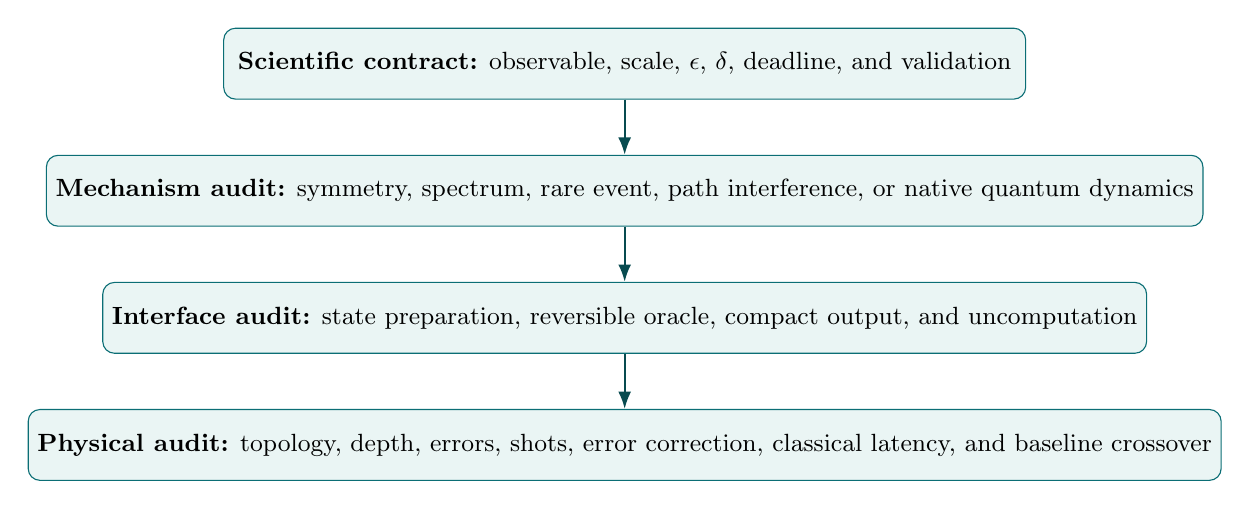
\begin{tikzpicture}[
  node distance=7mm,
  every node/.style={font=\small},
  box/.style={rounded corners=1.5mm,draw=quantum,fill=mist,minimum width=0.84\textwidth,minimum height=9mm,align=center},
  arrow/.style={-{Latex[length=2.2mm]},thick,draw=quantumdark}
]
\node[box] (contract) {\textbf{Scientific contract:} observable, scale, $\epsilon$, $\delta$, deadline, and validation};
\node[box,below=of contract] (structure) {\textbf{Mechanism audit:} symmetry, spectrum, rare event, path interference, or native quantum dynamics};
\node[box,below=of structure] (interface) {\textbf{Interface audit:} state preparation, reversible oracle, compact output, and uncomputation};
\node[box,below=of interface] (budget) {\textbf{Physical audit:} topology, depth, errors, shots, error correction, classical latency, and baseline crossover};
\draw[arrow] (contract) -- (structure);
\draw[arrow] (structure) -- (interface);
\draw[arrow] (interface) -- (budget);
\end{tikzpicture}
\caption{The order of operations for a credible quantum research program. A circuit is designed only after the scientific and interface contracts are explicit.}
\label{fig:order}
\end{figure}

\subsection{Define the output before the state}

The output contract is the fastest way to expose a weak proposal. Quantum algorithms are naturally good at returning a sample, a phase, an expectation value, a low-dimensional statistic, a property, or a candidate that can be verified classically. They are generally poor at returning every entry of a large vector. The Harrow--Hassidim--Lloyd algorithm is the canonical warning: it prepares a state proportional to the solution of a structured linear system and efficiently estimates appropriate observables; it does not print an $N$-component solution in polylogarithmic time \citep{harrow2009}. Reading $N$ classical numbers still costs at least order $N$.

Before selecting an encoding, the researcher should answer four questions.

\begin{enumerate}
  \item What single scientific decision will be made from the output?
  \item Is the desired output a scalar, sample, property, witness, ranked list, or full object?
  \item How will correctness be checked when exact classical simulation is no longer available?
  \item What level of approximation changes the scientific conclusion rather than merely the last decimal place?
\end{enumerate}

The last question matters because precision is a resource. An algorithm with complexity $O(1/\epsilon)$ can be theoretically superior to a classical $O(1/\epsilon^2)$ Monte Carlo method, but not necessarily at the $\epsilon$ required by the application once constants, state preparation, and fault tolerance are included. ``Faster in precision'' is not the same as ``faster by Friday.''

\subsection{Define the classical opponent honestly}

The baseline is not brute force unless brute force is what competent practitioners actually use. A quantum optimization method should meet mixed-integer programming, constraint programming, local search, decomposition, learned heuristics, and GPU implementations on the same instance distribution. A quantum simulation proposal should meet tensor networks, Monte Carlo, perturbation theory, reduced models, and high-performance computing in the regime where each is strongest. A quantum machine-learning claim should meet compressed, randomized, kernel, and quantum-inspired classical methods. Tang's dequantization of recommendation-system speedups remains an important engineering lesson: strong quantum input assumptions may grant a classical competitor more power as well \citep{tang2019,tang2021}.

The comparison must fix the same problem size $N$, accuracy $\epsilon$, confidence $1-\delta$, hardware budget, preprocessing, and acceptable output. Only then does the desired inequality have meaning:
\begin{equation}
T_Q(N,\epsilon,\delta;\Lambda)+T_{\mathrm{interface}}
<T_C(N,\epsilon,\delta;B_C).
\label{eq:crossover}
\end{equation}

\paragraph{Baseline protocol.} ``Strongest relevant classical baseline'' becomes operational only when the comparison is specified in advance:
\begin{enumerate}
  \item name the classical implementations (solver, version, and configuration) that practitioners currently use for this problem class, including at least one state-of-the-art heuristic and one exact or certified method where feasible;
  \item grant both sides identical preprocessing, instance distributions, and hardware budgets (including graphics processing units for the classical side);
  \item give the classical side a tuning budget equal to the quantum side's calibration and transpilation effort;
  \item compare at the same $(\epsilon,\delta)$ and the same output contract, reporting time-to-solution distributions rather than best cases;
  \item state which costs are amortized on each side and over how many uses.
\end{enumerate}

% !TeX root = ../../../main.tex
\section{Mechanisms That Illuminate a Quantum Opportunity}\label{sec:mechanisms}

Quantum advantage is not a substance sprinkled over a difficult problem. It comes from a mechanism. The most useful early question is therefore: \emph{what mathematical feature would make interference do less work than classical enumeration, simulation, or sampling?}

\begin{longtable}{>{\raggedright\arraybackslash}p{0.19\textwidth} >{\raggedright\arraybackslash}p{0.23\textwidth} >{\raggedright\arraybackslash}p{0.26\textwidth} >{\raggedright\arraybackslash}p{0.19\textwidth}}
\caption{Problem structure, quantum mechanisms, and the questions that decide whether the match is real.}\label{tab:mechanisms}\\
\toprule
\textbf{Structure in the problem} & \textbf{Quantum mechanism} & \textbf{Useful output} & \textbf{Decisive caveat}\\
\midrule
\endfirsthead
\toprule
\textbf{Structure in the problem} & \textbf{Quantum mechanism} & \textbf{Useful output} & \textbf{Decisive caveat}\\
\midrule
\endhead
Periodicity or group symmetry & Quantum Fourier transform, phase estimation, hidden-subgroup methods & Period, eigenphase, symmetry label & Is the function available coherently and is the promised structure present?\\
\addlinespace
Rare marked states in an unstructured space & Amplitude amplification or Grover search & A marked candidate or amplified event & The predicate must be reversible; total cost is repeated oracle cost, not only $\sqrt{N}$.\\
\addlinespace
Mean, probability, risk, or integral & Amplitude estimation & Scalar estimate & Preparation and reflections must be cheap enough; low-depth variants trade speedup for robustness.\\
\addlinespace
Spectral property of an operator & Phase estimation, qubitization, quantum signal processing & Energy, eigenphase, response function & Initial-state overlap, block encoding, precision, and coherent depth often dominate.\\
\addlinespace
Sparse, structured, well-conditioned linear system & Quantum linear-system algorithms or quantum singular value transformation (QSVT) & State or observable associated with the solution & Condition number, input oracle, and output tomography can erase the headline speedup.\\
\addlinespace
Local transitions, hitting, or collision structure & Quantum walks & Hitting time, collision, sampled endpoint & The graph access model and setup cost must be physically implementable.\\
\addlinespace
Native quantum dynamics & Digital or analog quantum simulation & Local observables, spectra, scattering data, correlation functions & State preparation, truncation, and validation replace classical data loading as the main risks.\\
\addlinespace
Constrained objective with useful geometry & Quantum approximate optimization algorithm (QAOA), alternating operators, annealing & Good feasible candidate or distribution & A QUBO is not evidence of advantage; mixers, embedding, optimizer cost, and classical heuristics matter.\\
\addlinespace
Classically hard output distribution & Sampling and interference experiments & Samples, moments, or a certified statistic & Practical value and scalable verification must be demonstrated separately from sampling hardness.\\
\bottomrule
\end{longtable}

\subsection{Interference as the operational design lever}

Superposition enlarges the state space. Entanglement creates correlations unavailable to product states. Neither fact alone tells us why an answer becomes easier, and the question of which resource ``powers'' quantum speedups is genuinely model-dependent: coherence, entanglement, contextuality, and magic each play the leading role in different formal accounts. This paper makes a narrower, operational claim: in gate-model algorithm \emph{design}, interference is where selectivity is engineered. The design task is to assign phases and amplitudes so that computational paths supporting the desired global property reinforce one another while irrelevant paths cancel.

For a reversible Boolean predicate $\chi(f(x))$, the basic compute--mark--uncompute pattern is
\begin{equation}
\ket{x}\ket{0}
\longrightarrow \ket{x}\ket{f(x)}
\longrightarrow (-1)^{\chi(f(x))}\ket{x}\ket{f(x)}
\longrightarrow (-1)^{\chi(f(x))}\ket{x}\ket{0}.
\label{eq:uncompute}
\end{equation}
The final arrow is not housekeeping. Garbage left entangled with $x$ can reveal which path was taken and destroy the interference the algorithm needed. Reversibility turns ordinary software concerns into algorithmic resources: temporary storage becomes ancilla count; irreversible updates become additional arithmetic; dynamic branches become controlled operations; and memory access becomes a circuit.

\subsection{Five gates before a research proposal earns a score}

It is tempting to assign every candidate a weighted ``quantum opportunity score.'' That creates false precision. A better process uses five gates. A proposal proceeds only if each gate has an explicit answer.

\begin{enumerate}
  \item \textbf{Mechanism gate.} Which known quantum primitive exploits a named property of the problem?
  \item \textbf{Access gate.} How are data, coefficients, Hamiltonian terms, or graph neighborhoods supplied coherently, and at what cost?
  \item \textbf{Output gate.} Is the deliverable compact enough to measure without reconstructing the whole state?
  \item \textbf{Physical gate.} Does the compiled computation fit the qubits, topology, error budget, coherence, throughput, and wall-clock bound?
  \item \textbf{Evidence gate.} Can the claim be falsified against strong classical baselines and validated beyond the classically simulable regime?
\end{enumerate}

If the access or output gate fails, a beautiful internal circuit is usually irrelevant. If the evidence gate fails, the project may still be good physics, compiler research, or device science, but it should not be sold as an application advantage.

\begin{warningbox}[Signals that are not sufficient]
The following facts do not, by themselves, identify a quantum opportunity: the dataset is large; the problem is NP-hard; a qubit can encode the variables; the state is entangled; the objective can be written as a QUBO; a toy circuit beats brute force; or the Hilbert space has dimension $2^n$. Hardness is a reason to look for structure. It is not the structure.
\end{warningbox}


% Phase II: compile the idea into a complete, falsifiable experiment.
\part{Engineering the Complete Experiment}
% !TeX root = ../../../main.tex
\section{Calculating a Research Question on a Physical Quantum Computer}\label{sec:resources}

Suppose a researcher has a physical machine, a scientific observable, and fixed bounds. How should she calculate whether the experiment is possible? She should begin by treating the machine as a resource envelope rather than a qubit count.

\subsection{The resource envelope}

For a gate-model processor, define
\begin{equation}
\Lambda_{\mathrm{HW}}=
\bigl(Q_{\mathrm{phys}},G_{\mathrm{native}},\mathcal{G}_{\mathrm{conn}},
p_{1},p_{2},p_m,p_{\mathrm{idle}},
\tau_{1},\tau_{2},\tau_m,T_1,T_2,
r_{\mathrm{reset}},\ell_C\bigr),
\end{equation}
where $Q_{\mathrm{phys}}$ is the available physical-qubit count, $G_{\mathrm{native}}$ the native gate set, $\mathcal{G}_{\mathrm{conn}}$ the coupling graph, $p$ and $\tau$ the error rates and durations of operations, $T_1$ and $T_2$ the coherence scales, $r_{\mathrm{reset}}$ the reset rate, and $\ell_C$ the latency of classical control, decoding, and network round trips. Calibration statistics should include distributions and drift, not only daily averages.

The algorithmic ledger should include, at minimum,
\begin{equation}
R_{\mathrm{alg}}=
\bigl(Q_L,N_{1q},N_{2q},D_{2q},N_M,N_T,D_T,N_{\mathrm{oracle}},
N_{\mathrm{shots}},N_{\mathrm{iter}},W_{\mathrm{classical}}\bigr).
\end{equation}
Here $D_{2q}$ is usually more revealing than total gate count on a noisy device, while $N_T$ and $D_T$ often dominate a surface-code fault-tolerant design because non-Clifford operations require distilled resource states \citep{fowler2012,gidney2021,vandam2024}.

\subsection{Spend error like a budget}

Fix an error metric for the reported quantity (for example, additive error on a normalized expectation value). The permitted scientific error should then be \emph{allocated} before implementation: choose targets $\bar\epsilon_i$ for each source such that their sum respects the requirement, and verify that each achieved contribution stays within its allocation. Two inequalities are needed, not one:
\begin{equation}
\epsilon_{\mathrm{achieved}}
\;\leq\;
\underbrace{\epsilon_{\mathrm{model}}
+\epsilon_{\mathrm{discretization}}
+\epsilon_{\mathrm{encoding}}
+\epsilon_{\mathrm{synthesis}}
+\epsilon_{\mathrm{statistical}}
+\epsilon_{\mathrm{hardware}}}_{\textstyle\sum_i \epsilon_i}
\;\leq\;
\epsilon_{\mathrm{target}}.
\label{eq:error-budget}
\end{equation}
The left inequality is the worst-case triangle bound; the right inequality is the budget constraint $\sum_i\bar\epsilon_i\leq\epsilon_{\mathrm{target}}$ that the design must satisfy by construction. Additivity is itself an assumption: correlated systematic errors can exceed the sum of individually characterized terms, while independent zero-mean statistical contributions combine in quadrature and make the triangle bound pessimistic. State which regime applies to each pair of terms.

Failure probabilities follow the same discipline through an explicit union bound. If the workflow can fail in stages $i$ (state preparation, logical faults, magic-state distillation, rotation synthesis, optimization failure, hypothesis testing) with probabilities $\delta_i$, then
\begin{equation}
\Pr[\text{any stage fails}]\;\leq\;\sum_i \delta_i\;\leq\;\delta_{\mathrm{target}},
\label{eq:delta-union}
\end{equation}
and each $\delta_i$ must be allocated before the stage is engineered. This is not clerical accounting. If the physics model already consumes the tolerance, improving gate fidelity cannot rescue the scientific result. If sampling consumes the wall-clock budget, shortening the circuit may not matter.

\subsection{A toy triage model for noisy devices}

For a shallow physical circuit, a deliberately crude screen assumes that every operation is followed by an \emph{independent stochastic Pauli fault} with the quoted probability, so the probability that no fault occurs anywhere is
\begin{equation}
P_{0}\approx
(1-p_{1})^{N_{1q}}
(1-p_{2})^{N_{2q}}
(1-p_m)^{N_M}
\exp\!\left(-\frac{T_{\mathrm{circ}}}{T_{\mathrm{coh}}}\right).
\label{eq:nisq-screen}
\end{equation}
This is a toy triage model, not a fidelity estimate. Its assumptions fail in specific, known ways: benchmark numbers such as randomized-benchmarking infidelities average over gate ensembles and cannot simply be substituted as per-location fault probabilities; coherent errors can add in amplitude rather than probability; crosstalk and leakage are not local; and the coherence exponential can double-count decay already reflected in the gate infidelities. The model is useful only in one direction: if this \emph{optimistic} calculation is already catastrophic, the circuit must change before a more expensive noise study. For a serious worked example, a channel-level simulation with a calibrated noise model should replace \cref{eq:nisq-screen}.

Measurement then sets a separate lower bound. For an observable whose per-shot outcome is bounded in $[-1,1]$ (range 2), Hoeffding's inequality gives
\begin{equation}
N_{\mathrm{shots}}
\geq \frac{2\ln(2/\delta)}{\epsilon_{\mathrm{statistical}}^2},
\label{eq:hoeffding}
\end{equation}
about $7.4\times10^{4}$ shots at $\epsilon=0.01$, $\delta=0.05$. When the variance $\sigma^2$ is known or estimated, a normal approximation gives
\begin{equation}
N_{\mathrm{shots}}\approx
\frac{z_{1-\delta/2}^{2}\sigma^2}{\epsilon_{\mathrm{statistical}}^2}.
\end{equation}
Measurement grouping, classical shadows, importance allocation, and problem symmetry can reduce the number of distinct circuits. Error mitigation can reduce bias, but it generally increases variance and sampling cost; its overhead must be measured rather than described as free cleanup \citep{cai2023,quek2024}.

If one run returns a valid solution with probability $p_s$ (assumed stationary across repetitions; drift violates this, see \cref{sec:evidence}), the repetitions required to succeed with probability at least $\eta$ are
\begin{equation}
R_{\eta}=\left\lceil
\frac{\ln(1-\eta)}{\ln(1-p_s)}
\right\rceil,
\qquad
\TTS_{\eta}=R_{\eta}
\left(T_Q+T_C+T_{\mathrm{I/O}}\right).
\label{eq:tts}
\end{equation}
Time-to-solution ($\TTS$), not gate count, is the honest unit for a probabilistic hybrid workflow.

\subsection{Worked noisy example: the circuit fits, but does the experiment?}

Consider a hypothetical 40-qubit expectation-value experiment with $N_{1q}=600$, $N_{2q}=300$, $N_M=40$, $p_1=2\times10^{-4}$, $p_2=5\times10^{-3}$, $p_m=1.5\times10^{-2}$, and $T_{\mathrm{circ}}/T_{\mathrm{coh}}=0.15$. The screening model gives
\begin{align}
\ln P_0 &\approx 600\ln(0.9998)+300\ln(0.995)
+40\ln(0.985)-0.15\\
&\approx -2.38,
\end{align}
or $P_0\approx 0.093$. That does not mean $9.3\%$ of shots are labeled ``correct.'' It means the no-fault path is already rare under an optimistic model, so the observable must be unusually noise-robust, symmetry-verifiable, or shallow enough after recompilation to justify hardware time.

Now consider the measurement budget for an energy estimate, done properly. Write the Hamiltonian as $H=\sum_j c_j P_j$ with Pauli terms $P_j$ partitioned into $G$ commuting groups; group $g$ carries weight $a_g=\sum_{j\in g}\lvert c_j\rvert$, and each shot of setting $g$ returns a value in $[-a_g,a_g]$. The estimator is $\hat H=\sum_g \hat\mu_g$ with per-group sample means $\hat\mu_g$, so
\begin{equation}
\Var(\hat H)=\sum_{g=1}^{G}\frac{\sigma_g^2}{N_g},
\qquad \sigma_g^2\leq a_g^2,
\label{eq:grouped-variance}
\end{equation}
where covariances between groups vanish because settings are measured in separate shots. It is \emph{not} sufficient to give every setting the single-observable shot count from \cref{eq:hoeffding}: that controls each $\hat\mu_g$ separately but says nothing about the total error of $\hat H$ at joint confidence $1-\delta$. Two correct allocations bracket the answer.

\emph{Worst-case allocation.} Allocate the error budget as $\epsilon_g=\epsilon\, a_g/\sum_h a_h$ and the failure budget uniformly, $\delta_g=\delta/G$ (union bound, \cref{eq:delta-union}). Hoeffding on each group then requires
\begin{equation}
N_g\geq \frac{2a_g^2\ln(2G/\delta)}{\epsilon_g^2}
=\frac{2\bigl(\sum_h a_h\bigr)^2\ln(2G/\delta)}{\epsilon^2}.
\label{eq:worstcase-shots}
\end{equation}
For $G=40$ groups with total weight $\sum_h a_h=1$ (declared toy normalization), $\epsilon=0.01$, and $\delta=0.05$, this gives $N_g\approx1.5\times10^{5}$ per setting and roughly $5.9\times10^{6}$ shots per energy evaluation---about 3.3 hours of raw QPU time per optimizer step at an \emph{assumed} 2 ms per shot (shot time is platform-dependent by orders of magnitude, and total time scales linearly in it).

\emph{Variance-aware allocation.} If group variances $\sigma_g^2$ are measured, Neyman allocation $N_g\propto\sigma_g$ under a normal approximation gives a total
\begin{equation}
N_{\mathrm{shots}}\approx
\frac{z_{1-\delta/2}^{2}\bigl(\sum_g \sigma_g\bigr)^2}{\epsilon^2},
\label{eq:neyman-shots}
\end{equation}
which for the same toy weights with $\sigma_g$ near their bound is roughly $3.8\times10^{4}$ shots---about 1.3 minutes per evaluation---and far less when the state concentrates the variance in a few groups. The two estimates do not carry the same guarantee: \cref{eq:worstcase-shots} is finite-sample and distribution-free, while \cref{eq:neyman-shots} is asymptotic, holds the \emph{total} error to $\epsilon$ only approximately, and requires variances from a pilot run whose $G N_{\mathrm{pilot}}$ shots (and per-group rounding $\lceil N_g\rceil$) belong in the ledger. In the reproducible demonstration of \cref{app:demo}, the worst-case allocation achieved empirical coverage $1.000$ and the Neyman allocation $0.955$ against a $0.95$ target---exactly the expected behavior of a bound versus an approximation. The roughly $150\times$ spread between \cref{eq:worstcase-shots,eq:neyman-shots} is the point: measured variances, coefficient weighting, and an explicit joint-confidence argument are not refinements, they are the calculation. Twenty optimizer evaluations range from under an hour to several days depending on which regime the instance occupies, before queueing, compilation, calibration circuits, or mitigation. The real research question has changed from ``Does the 40-qubit circuit fit?'' to ``Can structure reduce settings, variance, or iterations by an order of magnitude without biasing the observable?'' That is a useful question. All numbers in this subsection are reproduced by \texttt{scripts/verify\_calculations.py} in the paper's artifact.

\subsection{Fault-tolerant calculation}

For an error-corrected machine, let $L$ be the number of fault locations and allocate logical failure probability $\delta_{\mathrm{QEC}}$. A common surface-code engineering model is
\begin{equation}
p_L(d)\approx A\left(\frac{p}{p_{\mathrm{th}}}\right)^{(d+1)/2},
\label{eq:logical-error}
\end{equation}
which captures exponential suppression below threshold. Recent below-threshold surface-code experiments report this scaling form while also exposing correlated-error floors and real-time decoding demands \citep{acharya2025}. Requiring $L p_L(d)\leq\delta_{\mathrm{QEC}}$ gives the screening distance
\begin{equation}
d\geq
2\frac{\ln\!\left(\delta_{\mathrm{QEC}}/(A L)\right)}
{\ln\!\left(p/p_{\mathrm{th}}\right)}-1,
\label{eq:distance}
\end{equation}
rounded up to a supported code distance. The physical-qubit count is then approximately
\begin{equation}
Q_{\mathrm{phys}}
\approx c_d d^2 Q_L+Q_{\mathrm{factory}}+Q_{\mathrm{routing}}+Q_{\mathrm{buffer}},
\label{eq:physical-qubits}
\end{equation}
where $c_d$ is a layout constant (about 2 for a rotated surface-code patch, larger once operational layout and lattice-surgery ancillas are included). The runtime is bounded below by both logical dependency depth and magic-state supply:
\begin{equation}
T_{\mathrm{run}}\gtrsim
\max\!\left(D_{\mathrm{dep}}\tau_L,\frac{N_T}{R_T}\right)
+T_{\mathrm{decode}}+T_{\mathrm{feedforward}},
\label{eq:ft-runtime}
\end{equation}
where $D_{\mathrm{dep}}$ is the depth of the logical dependency graph and $\tau_L$ is the logical cycle time, itself roughly $d$ rounds of syndrome extraction plus decoding latency.

As an illustration, take $L=10^{10}$, $\delta_{\mathrm{QEC}}=10^{-2}$, $A=0.1$, and $p/p_{\mathrm{th}}=0.1$. Equation \eqref{eq:distance} gives $d\geq21$. The idealized rotated surface-code memory count $2d^2-1$ is then 881 physical qubits per logical qubit, so a 1,000-logical-qubit algorithm begins near 881,000 physical qubits. This figure is an \emph{idealized memory-only floor}: it excludes operational patch layout, lattice surgery routing, distillation factories, spare capacity, and control infrastructure, each of which typically multiplies the count. The estimate is also steeply sensitive to its inputs---halving $p/p_{\mathrm{th}}$ or relaxing $\delta_{\mathrm{QEC}}$ by an order of magnitude changes $d$ by several steps and the qubit count quadratically in $d$, while factory count and logical cycle time trade against each other in \cref{eq:ft-runtime}. A publishable estimate should therefore report a sensitivity table over physical error rate, error budget, code distance, factory count, and logical cycle time, ideally produced by an established resource estimator rather than by \cref{eq:distance,eq:physical-qubits} alone. Modern tools explicitly combine physical error rates, operation times, quantum error correction (QEC) protocols, error budgets, logical depth, and distillation constraints for this reason \citep{beverland2022,vandam2024}.

We ran exactly this check, with one framing caveat stated up front: the input is a \emph{synthetic sensitivity scenario}, not a compiled algorithm. The screening scenario above---1{,}000 logical qubits with $L=10^{10}$ fault locations, modeled as a $T$-count-dominated workload ($T$-count $10^{10}$)---was passed through the Azure Quantum Resource Estimator \citep{beverland2022}, executed locally, sweeping four qubit models and three total error budgets ($10^{-1}$, $10^{-2}$, $10^{-3}$). No algorithmic trace backs the $10^{10}$ figure, so the outputs quantify how the tool's layered models respond to inputs of this magnitude; a publishable \emph{application} estimate requires an actual logical circuit. Within that scope, the sweep corrects the hand calculation in two instructive directions. First, the tool's layout model assigns 2{,}091 algorithmic logical qubits rather than 1{,}000: routing and ancilla space roughly double the logical footprint before any code distance is chosen (a model-dependent output, not an absolute correction). Second, the physical totals bracket rather than confirm the 881{,}000-qubit memory-only floor: a superconducting-style gate model at $p=10^{-3}$ needs code distance 27--31 and \emph{3.4--4.7 million} physical qubits with runtimes over a day, while the same workload at $p=10^{-4}$ needs distance 13--15 and 0.79--1.16 million qubits in 14--17 hours, and an aggressive Majorana model at $p=10^{-6}$ drops to distance 7 and roughly 0.54--0.81 million qubits in under six hours. One order of magnitude in physical error rate moves the answer by roughly $6\times$ in qubits and $5\times$ in runtime; the error budget moves it by tens of percent. The complete sweep, including $T$-factory counts and the exact tool inputs, is archived in the reproducibility artifact (\texttt{artifacts/estimator/}). The lesson stands: the single impressive integer from \cref{eq:distance,eq:physical-qubits} was neither an upper nor a lower bound, and only a tool run with a declared machine model, a real logical workload, and a sensitivity table is publishable.

\begin{warningbox}[What the algebra does not know]
Equations \eqref{eq:logical-error}--\eqref{eq:ft-runtime} are planning models, not warranties. Long-range correlated events, leakage, decoder latency, yield, fabrication variation, thermal constraints, network congestion, and control electronics can dominate a real architecture. A resource estimate should therefore be published with its machine model and sensitivity analysis, not as a single impressive integer.
\end{warningbox}

% !TeX root = ../../../main.tex
\section{The Experimental Program: Make the Claim Falsifiable}\label{sec:evidence}

A quantum algorithm paper becomes more valuable when the experiment is designed to prove the authors wrong. The following protocol treats validation as part of the algorithm.

\subsection{Predeclare the success condition}

Before running the device, record the primary observable, error tolerance, confidence level, time limit, resource accounting rules, baseline implementations, and stopping rule. If the goal is solution quality, specify the approximation ratio or constraint violation. If the goal is a physical observable, specify the acceptable total error and how model error will be separated from hardware error. If the goal is runtime, include preprocessing, queueing assumptions, repeated shots, calibration, mitigation, and classical postprocessing.

Benchmark suites improve comparability only when the abstraction level and compilation assumptions are visible \citep{quetschlich2023}. The result should be reproducible from a manifest containing the device identifier, calibration snapshot, coupling map, native gate set, compiler and optimization levels, seeds, shot allocation, mitigation settings, raw counts, classical hardware, code commit, and wall-clock timestamps.

\subsection{Use an instance ladder}

One large instance teaches surprisingly little. A useful ladder contains:

\begin{enumerate}
  \item \textbf{Exact instances}, small enough for full-state simulation and symbolic checks.
  \item \textbf{Mechanism instances}, constructed so the proposed symmetry, periodicity, gap, or rare-event structure can be turned on and off.
  \item \textbf{Application instances}, drawn from the real distribution without selecting only favorable examples.
  \item \textbf{Stress instances}, targeting poor conditioning, small spectral gaps, dense constraints, adversarial noise sensitivity, or weak initial overlap.
  \item \textbf{Crossover instances}, large enough to test scaling but still comparable with the best available classical method.
\end{enumerate}

The mechanism-off control is especially important. If performance does not change when the alleged quantum structure is removed, the proposed explanation is probably wrong even if the benchmark score is good.

\subsection{Separate four kinds of evidence}

The experiment should not collapse correctness, scaling, utility, and advantage into one plot.

\begin{itemize}
  \item \textbf{Correctness evidence}: agreement with exact values, conserved quantities, symmetries, or certified bounds.
  \item \textbf{Mechanism evidence}: response to ablations that remove the feature the quantum algorithm claims to exploit.
  \item \textbf{Scaling evidence}: fitted resource growth with uncertainty across instance families, including compiler and sampling costs.
  \item \textbf{Advantage evidence}: end-to-end comparison with a strong classical baseline at matched accuracy and confidence.
\end{itemize}

Quantum certification becomes harder when classical simulation fails, so scalable checks must be designed early: conserved charges, variational upper bounds, local consistency conditions, cross-entropy-style statistics where appropriate, trap circuits, interactive proofs, or agreement among independent formulations \citep{eisert2020}. ``The simulator could not run it'' is evidence of size, not correctness.

\subsection{Treat drift as an experimental variable}

Run interleaved controls, randomize execution order, repeat across calibration windows, and report between-window variance. A device can improve during one part of a benchmark and worsen during another. Without interleaving, time becomes an unacknowledged confounder. Likewise, error mitigation should be trained and evaluated on separated circuits when possible; tuning on the final answer converts validation into fitting.

% !TeX root = ../../../main.tex
\section{Where the Quantum Side Ends: Designing the Hybrid Boundary}\label{sec:hybrid}

The quantum--classical boundary is not a philosophical line. It is a costed interface. Let a partition $\Pi$ assign subroutines to the classical processor, QPU, or shared workflow. A reasonable design objective is
\begin{equation}
\Pi^*=\arg\min_{\Pi}
\left[
T_C(\Pi)+T_{\mathrm{transfer}}(\Pi)+T_Q(\Pi)
\right]
\label{eq:partition}
\end{equation}
subject to bounds on total error, qubits, coherence, memory, success probability, energy, and deadline. Transfer includes data encoding, circuit submission, measurement, serialization, latency, and reinitialization. If a small quantum kernel must be called millions of times through a slow interface, its asymptotic elegance may become a systems failure.

\begin{table}[htbp]
\centering
\small
\caption{A practical partition rule for hybrid algorithms.}
\label{tab:hybrid}
\begin{tabularx}{\textwidth}{>{\bfseries\raggedright\arraybackslash}p{0.20\textwidth} X X}
\toprule
Facet & Prefer the classical side & Consider the quantum side\\
\midrule
Data & Large explicit datasets, parsing, cleaning, sparse indexing, branching & Quantum-native states or compact generative preparation circuits\\
Control & Irregular logic, dynamic memory, high-precision bookkeeping & Coherent control that is essential to interference\\
Computation & Cheap arithmetic, preprocessing, decomposition, warm starts & Spectral transforms, amplitude amplification, coherent evolution\\
Constraints & Presolve, propagation, cutting planes, feasibility repair & Constraint-preserving mixers or symmetry sectors that remove invalid states\\
Optimization & Global orchestration, stopping rules, surrogate models & Sampling or expectation evaluation only when it adds nonclassical information\\
Output & Full vectors, reports, databases, provenance & Compact observables, samples, phases, witnesses, candidate solutions\\
Validation & Baselines, confidence intervals, residuals, cross-checks & Conserved quantities or quantum tests unavailable classically\\
\bottomrule
\end{tabularx}
\end{table}

\subsection{The reusable-kernel rule}

The QPU should receive the smallest kernel that (1) requires coherence, (2) is expensive classically, (3) can be invoked without repeatedly loading a giant state, and (4) returns a compact object. Classical preprocessing should expose structure rather than merely shrink data. Examples include finding symmetry sectors, eliminating fixed variables, constructing a sparse block encoding, preparing a warm start, grouping observables, or decomposing a graph into neighborhoods.

The strongest hybrid algorithms often do not divide the original problem in half. They change the problem so that a narrow quantum operation becomes meaningful. The quantum step may estimate a phase, generate a distribution, evaluate a correlation, or search a residual space after classical presolve. Everything else remains classical because classical computers are excellent at memory, branching, precision, and control.

\subsection{Variational algorithms: useful laboratory, dangerous default}

Variational quantum algorithms place state preparation and expectation estimation on the QPU while a classical optimizer updates parameters \citep{peruzzo2014,cerezo2021}. This is experimentally convenient, but convenience is not a mechanism. Expressive ansatze can exhibit exponentially small gradients, while noise can create its own barren plateaus \citep{mcclean2018,wang2021}. The optimizer may spend more time estimating a flat landscape than exploring it.

A variational design should therefore justify the ansatz from problem structure, preserve known symmetries, measure gradient signal-to-noise, report the number of objective calls, and compare against a classical ansatz with similar inductive bias. If the circuit is classically simulable because it is shallow or weakly entangling, that may be a good engineering property during development, but it weakens an advantage claim. If it is deep enough to resist simulation, trainability and noise become harder. The tension is real and must be addressed in the design, not deferred.

% !TeX root = ../../../main.tex
\section{What Engineering Has Already Identified}

Across algorithms and hardware, several principles now repeat often enough to be treated as engineering knowledge.

\subsection{Hard is not a mechanism}

NP-hardness identifies a worst-case classical complexity class. It does not promise a quantum speedup, much less a near-term one. Grover search offers a quadratic improvement for black-box search, not an exponential escape from arbitrary combinatorial structure \citep{grover1997}. Useful quantum optimization requires additional geometry, spectral properties, instance distributions, or constrained dynamics.

\subsection{Input models are part of the theorem}

Oracle access, quantum random-access memory (QRAM), sparse access, block encodings, and amplitude-encoded states are not equivalent. Their construction cost can determine the application. Conversely, structured data may sometimes be prepared by compact circuits, so ``loading is always linear'' is also too crude. The researcher must state the access model and compile it for the actual data distribution rather than argue by slogan \citep{aaronson2015,tang2021}.

\subsection{Output size can reverse a speedup}

An $n$-qubit state can hold quantities whose classical description would be exponentially large, but measurement returns at most $n$ bits per shot: the state is a compact \emph{carrier} of certain global properties, not a readable database. Prefer questions whose answer is a statistic, energy, phase, sample, classification, or verifiable candidate. If the downstream system requires every amplitude, put the readout cost in the theorem.

\subsection{Asymptotics need a crossover}

Big-$O$ notation removes constants, yet constants are where fault tolerance lives. Resource studies repeatedly show that an asymptotically superior method can lose at all practical input sizes, or require a logical clock rate and physical-qubit count that move the crossover beyond the scientific deadline \citep{gidney2021,vandam2024}. Publish the crossover surface over $N$, $\epsilon$, physical error rate, and hardware throughput, not a single curve with the inconvenient region cropped away.

\subsection{Compilation changes the algorithm}

Connectivity inserts swaps. Gate synthesis converts rotations into non-Clifford resources. Mid-circuit measurement adds feedforward latency. Routing increases idle errors. A logical circuit and a physical experiment are different artifacts; both should be versioned and costed.

\subsection{Error mitigation is sampling debt}

Mitigation can turn a biased estimate into a better one, but the bill often arrives as variance, additional circuits, model assumptions, and calibration sensitivity. Fundamental results limit the scalability of undoing generic noise without correction \citep{cai2023,quek2024}. The honest metric is error at fixed total experimental cost.

\subsection{Constraints can become architecture}

Penalty terms are not the only way to handle constraints. If a mixer or encoding remains inside the feasible subspace, invalid states never consume amplitude. Constraint-preserving constructions can reduce wasted search and improve interpretability, although their circuits may be more complex \citep{fuchs2024}. The constraint graph should shape the circuit, not merely punish it afterward.

\subsection{The classical frontier moves when quantum work exposes structure}

Quantum research frequently produces better classical algorithms, tensor-network approximations, randomized numerical methods, or improved decompositions. That is not failure. It is evidence that the problem has been understood more deeply. A credible program expects the baseline to fight back.


% Phase III: stress-test the framework against concrete domains.
\part{Application Stress Tests}
% !TeX root = ../../../main.tex
\section{Illustrative Engineering Audits}\label{sec:audits}

The two audits in this section apply the problem contract to proposed framings. They are audits, not completed case studies: no hardware execution, full formulation, or benchmarked baseline is reported here. A small, fully reproducible execution of the audit procedure---including a quantitative version of this section's phase-encoding rejection---appears in \cref{app:demo}; this section closes by specifying the hardware-scale demonstration that remains open.

\subsection{DNA in phase: representation is not yet a biological mechanism}

Suppose the four DNA bases are mapped to four phases on one qubit,
\begin{equation}
\ket{\psi_b}=\frac{1}{\sqrt{2}}
\left(\ket{0}+e^{i\phi_b}\ket{1}\right),
\qquad
\phi_b\in\left\{0,\frac{\pi}{2},\pi,\frac{3\pi}{2}\right\}.
\label{eq:dna-phase}
\end{equation}
The adjacent states are not orthogonal:
\begin{equation}
\braket{\psi_b}{\psi_c}
=\frac{1+e^{i(\phi_c-\phi_b)}}{2},
\qquad
\left|\braket{\psi_b}{\psi_c}\right|=\frac{1}{\sqrt{2}}
\end{equation}
for a quarter-turn separation. They cannot be perfectly distinguished in one measurement. Two distinct phases matter here and must not be conflated. A \emph{global} phase multiplying an entire state, $e^{i\alpha}\ket{\psi}$, is unobservable: no measurement distinguishes it. The $\phi_b$ in \cref{eq:dna-phase} are \emph{relative} phases between the $\ket{0}$ and $\ket{1}$ components and are physically meaningful---but only through interference, not through direct readout. And regardless of phase bookkeeping, four exact classical symbols require at least a four-dimensional orthogonal space, such as two qubits or a ququart.

That does not make phase encoding useless. It changes the question. A sequence
\begin{equation}
\ket{\Psi_S}=\frac{1}{\sqrt{N}}
\sum_{j=0}^{N-1}e^{i\phi(S_j)}\ket{j}
\label{eq:phase-sequence}
\end{equation}
carries the base identities as relative phases across position states $\ket{j}$, which interference can access. Applying the quantum Fourier transform and measuring yields frequency $k$ with probability
\begin{equation}
\Pr[k]=\frac{1}{N^{2}}\left|\sum_{j=0}^{N-1}e^{i\phi(S_j)}e^{-2\pi i jk/N}\right|^{2},
\end{equation}
so the device samples from the power spectrum of the phase sequence: strong periodicities appear as high-probability frequencies, and each run returns one sample, not the spectrum. A reversible motif score $s(j)$ may instead support a predicate $\chi(j)=[s(j)\geq\tau]$ and amplitude amplification. But the complete cost includes sequence access, score computation, comparison, phase marking, uncomputation, and repetition: preparing \cref{eq:phase-sequence} from classical sequence data costs $O(N)$ operations, and a classical fast Fourier transform (FFT) returns the \emph{entire} spectrum in $O(N\log N)$ with small constants, so the sampling picture alone does not win. The arithmetic at realistic scale is unforgiving: for a bacterial genome ($N\approx5\times10^{6}$) the state preparation alone costs on the order of $10^{7}$ quantum operations \emph{per sample}, while $N\log_2 N\approx10^{8}$ classical floating-point operations---well under a second on one commodity core---deliver every frequency at once; for the human genome ($N\approx3\times10^{9}$) the FFT remains a minutes-scale commodity computation, and reconstructing even a crude spectrum from quantum samples would require many complete state preparations. Absent a qRAM-like access model whose own physical cost is charged to the ledger (\cref{sec:hybrid}), the mechanism audit fails at the interface step for this encoding, independent of hardware quality. A per-method literature comparison against suffix-array and index-based motif search is left as future work rather than cited loosely here.

The more promising abstraction may be relational rather than symbolic---this is hypothesis generation, not a result. Folding, regulatory interaction, mutation pathways, and molecular geometry naturally produce graphs, Hamiltonians, local constraints, and energy landscapes. The researcher's job is to find the decisive observable: a spectral gap, transition amplitude, rare motif probability, or local correlation. The biological label is context. The operator is the algorithm.

\subsection{Scheduling and the QUBO temptation: a warning example}

This audit is included as a \emph{warning}, not as evidence that the framework improves scheduling: no benchmark is run here. For a scheduling problem, binary variables $x_{s,t,k}$ may indicate that satellite, instrument, or task $s$ is assigned at time $t$ under mode $k$. An objective can combine scientific reward, fuel, lateness, conflicts, and constraint penalties. To make the temptation concrete, consider the smallest honest instance class: $S$ tasks, $T$ time slots, one mode, at-most-one assignment per task, and at-most-one task per slot. The QUBO is
\begin{equation}
\min_{x\in\{0,1\}^{ST}}
\;-\!\sum_{s,t} r_{s,t}\,x_{s,t}
\;+\;\lambda\!\sum_{s}\Bigl(\sum_{t}x_{s,t}-1\Bigr)^{2}
\;+\;\lambda\!\sum_{t}\Bigl(\sum_{s}x_{s,t}-1\Bigr)^{2},
\label{eq:sched-qubo}
\end{equation}
which already exhibits every pathology in miniature. Feasibility requires the penalty weight to dominate the largest reward a single constraint violation can buy, $\lambda>\max_{s,t}r_{s,t}$; but on annealing-style hardware the couplings are rescaled into a fixed analog range, so every unit of $\lambda$ spent enforcing feasibility compresses the reward differences $r_{s,t}-r_{s',t'}$ that the optimizer must resolve, and the effective objective resolution degrades as $\max r/\lambda$. The quadratic penalties couple all $T$ variables of each task row and all $S$ variables of each slot column, so the QUBO graph contains $S+T$ cliques---dense structure that forces long embedding chains on sparse hardware graphs. And each additional real-world feature (multi-slot tasks, precedence, capacity) adds auxiliary variables quadratically. All of this is incurred \emph{before} any quantum mechanism is engaged; the assignment core of \cref{eq:sched-qubo} is solvable in polynomial time by bipartite matching, so the honest baseline destroys the naive formulation before the QPU is switched on.

A stronger workflow begins classically: eliminate impossible windows, merge equivalent states, decompose weakly coupled regions, generate feasible warm starts, and identify the residual choice that remains combinatorially expensive. The QPU then explores a structured neighborhood or feasible subspace, possibly with a constraint-preserving mixer, while the CPU repairs, certifies, and coordinates the global schedule. Quantum performance must be compared with CP-SAT (Google's constraint-programming/SAT solver), mixed-integer programming, local search, and domain heuristics using time-to-target and solution quality. Studies of the quantum approximate optimization algorithm (QAOA) already show that sampling frequency, circuit depth, and baseline choice determine the putative crossover \citep{lykhov2023}.

A practical intermediate artifact is an algorithm-opportunity and provenance record: each proposed quantum kernel records the claimed mechanism, access model, oracle cost, output contract, precision, logical resources, physical assumptions, noise sensitivity, classical baseline, verification method, and evidence status. This turns enthusiasm into an auditable engineering object. The version-pinned Ariadion toolchain used in \cref{app:demo} (repository and commit hash given there) is one host in which such records can live alongside executable circuits and their manifests.

\subsection{Toward an end-to-end demonstration}

The framework's own standard demands one completed pass. The demonstration that would qualify---deliberately small---is:

\begin{enumerate}
  \item \textbf{Problem contract:} a fully instantiated $\mathcal{P}$ for one bounded instance class. \emph{Done:} the frozen instance is the 4-qubit transverse-field Ising model of \cref{app:demo} ($J=1$, $g=1.2$, $\epsilon=0.1$, $\delta=0.05$), fixed before any execution.
  \item \textbf{Encoding and circuit:} explicit mapping, ansatz or algorithm choice, and compiled circuits for a named device with its calibration snapshot. \emph{Done at simulator scale:} the audit circuits were transpiled at optimization level 3 for IBM's Heron-class \texttt{torino} topology, and the transpiled QASM3 together with the device's measured calibration snapshot (per-gate error rates, $T_1$/$T_2$, readout error) is archived in \texttt{artifacts/hardware/}.
  \item \textbf{Resource calculation:} the full \cref{sec:resources} workflow---error budget, grouped shot budget with measured variances, noise triage, and a fault-tolerant estimate from an established resource estimator. \emph{Done:} Neyman-allocated shot budgets from measured variances (\cref{app:demo}); a calibration-derived Gate-4 screen ($P_0=0.940$ from the archived snapshot, versus $0.887$ from representative rates); and the Azure Quantum Resource Estimator sweep of \cref{sec:resources} (\texttt{artifacts/estimator/}).
  \item \textbf{Execution and measurement:} hardware or high-fidelity-simulator runs with predeclared analysis. \emph{Done at simulator scale:} seeded Aer runs reproduce the ideal energy within $0.7\sigma$; runs against a noise model built from real \texttt{torino} calibration data show the predicted noise bias ($\hat{E}=-4.490\pm0.026$ against $E_{\mathrm{ref}}=-4.654$, a $+0.164$ shift toward zero at $6.2\sigma$). Raw counts, job identifiers, and manifests are archived. \emph{Pending:} the same script's real-device path awaits queue access.
  \item \textbf{Classical baseline:} the protocol of \cref{sec:contract} against classical solvers on identical instances. \emph{Done:} an independent NumPy exact-diagonalization oracle, written without either quantum SDK, fixes $E_0$ and all reference distributions; both SDKs agree with it to $10^{-9}$.
  \item \textbf{Crossover decision:} the resulting go/no-go call with the complete ledger \eqref{eq:complete-ledger}, published with code and manifest. \emph{Done for this instance:} the decision is \emph{classical-only}---the instance is exactly solvable and the ledger says so; scripts, artifacts, and SHA-256 manifests are published in the paper's repository.
\end{enumerate}

The pass is complete at simulator scale with measured-calibration noise, and every artifact is archived; the single missing rung is a physical-device execution of the already-archived circuits, for which the pipeline is built and waiting. Until that run and a genuinely classically-hard instance exist, the framework should still be read as a proposed discipline demonstrated end-to-end only on a small exactly solvable instance---a falsifiable promissory note with its first installment paid.

% !TeX root = ../../../main.tex
\section{Subatomic Physics: Where Quantum Structure Is Native}\label{sec:hep}

Subatomic physics is one of the strongest \emph{conceptual} matches for quantum computation---in the mechanism sense of \cref{sec:mechanisms}, not as a claim of demonstrated practical advantage---because the expensive object is already quantum. Feynman's original argument was not that quantum computers should accelerate every database. It was that classical probability may fail to represent quantum physics efficiently, suggesting that a controllable quantum system should simulate another \citep{feynman1982}. Modern high-energy physics (HEP) and nuclear programs target Hamiltonian dynamics, lattice gauge theories, scattering, real-time response, finite-density physics, neutrino systems, and many-body structure \citep{bauer2023prx,bauer2023nrp,dimeglio2024}.

\subsection{Why the opportunity is real}

Classical lattice field theory is extraordinarily successful for equilibrium quantities in regimes compatible with importance sampling. The opportunity appears where classical methods encounter a sign problem, entanglement growth, real-time evolution, finite density, or exponentially large state spaces. A quantum processor can represent the state directly and apply local time evolution without enumerating all amplitudes. The mechanism is Hamiltonian simulation, not the phrase ``particle physics.''

For a lattice gauge calculation, the scientific error ledger may be written
\begin{equation}
\epsilon_{\mathrm{HEP}}
\leq
\epsilon_{\mathrm{lattice}}
+\epsilon_{\mathrm{volume}}
+\epsilon_{\mathrm{field\ trunc.}}
+\epsilon_{\mathrm{state\ prep.}}
+\epsilon_{\mathrm{time\ evol.}}
+\epsilon_{\mathrm{measurement}}
+\epsilon_{\mathrm{hardware}}.
\label{eq:hep-error}
\end{equation}
The continuum result requires reducing lattice spacing and increasing volume; bosonic fields or gauge links may require Hilbert-space truncation; physical scattering states must be prepared; Hamiltonian evolution must be approximated; and observables need repeated measurement. A tiny circuit with low hardware error can still answer the wrong field theory if the first three terms dominate.

Gauge symmetry illustrates how physics should shape the algorithm. Gauss's law can be enforced by a gauge-invariant encoding, a restricted basis, symmetry verification, or energy penalties. The first choices can reduce invalid states but complicate local operations; the penalty choice is simple but can distort energy scales and demand higher precision. Recent qudit experiments emphasize that matching hardware dimension and connectivity to gauge degrees of freedom can reduce encoding overhead \citep{meth2025}. Hardware--algorithm co-design changes the size of the physical Hilbert space here.

\subsection{A bounded subatomic research workflow}

For a question such as ``What is the real-time response $C(t)=\bra{\psi_0}O(t)O(0)\ket{\psi_0}$ within tolerance $\epsilon$ for a truncated lattice theory?'', the researcher should:

\begin{enumerate}
  \item specify the lattice, boundary conditions, gauge group, field truncation, initial state, observable, time window, and total error;
  \item exploit conserved charges and symmetries before mapping degrees of freedom to qubits or qudits;
  \item choose between product formulas, qubitization, variational dynamics, or analog simulation using the actual Hamiltonian structure and hardware regime;
  \item estimate state-preparation overlap and the cost of every SELECT/PREPARE oracle (the standard pair of subroutines used to block-encode a Hamiltonian as a linear combination of unitaries) or Trotter step;
  \item allocate shots according to observable variance and decide which local or symmetry checks remain classically verifiable;
  \item validate against exact diagonalization, tensor networks, perturbative limits, and Euclidean calculations on an instance ladder;
  \item extrapolate lattice, truncation, and hardware errors separately rather than fitting one forgiving curve.
\end{enumerate}

This is a strong \emph{mechanism match}---the representation, dynamics, and observable can all remain quantum---conditional on the interface and physical audits passing for a specific bounded model. It is also demanding because the scientific limit requires multiple simultaneous extrapolations. The match is strong; the schedule is not automatically short, and no practical advantage follows automatically from the dynamics being quantum-native.
% TODO: instantiate this workflow for a bounded model (e.g., a small Schwinger-model response function) with explicit truncation, budget, and baseline numbers, rather than leaving the checklist abstract.

% !TeX root = ../../../main.tex
\section{Astronomy: Separate the Sky, the Data Center, and the Sensor}\label{sec:astro}

Astronomy contains at least three distinct quantum opportunities, and combining them creates confusion.

\subsection{Classical astronomical data analysis}

Telescope images, catalogs, and interferometer time series are classical after detection. Quantum algorithms may help with search, inference, linear algebra, sampling, or optimization, but the access and output gates become severe. A quantum image representation that requires loading every pixel and reconstructing every output pixel has likely moved work rather than removed it. Radio-astronomy studies have therefore focused explicitly on comparing quantum encodings and toy reconstruction pipelines, which is the correct early question \citep{brunet2023}.

Gravitational-wave matched filtering is a cleaner mechanism example. After detection, the data are classical, and the physically correct statistic is noise-weighted: given detector data $d$ with one-sided noise power spectral density (PSD) $S_n(f)$---the frequency-resolved variance of the detector noise---and a bank of $M$ waveform templates $h_j$, the inner product is
\begin{equation}
\langle d,h_j\rangle
=4\,\mathrm{Re}\!\int_{0}^{\infty}
\frac{\tilde{d}(f)\,\tilde{h}_j^{*}(f)}{S_n(f)}\,df,
\qquad
\rho_j=\frac{\langle d,h_j\rangle}{\sqrt{\langle h_j,h_j\rangle}},
\label{eq:gw-snr}
\end{equation}
where tildes denote Fourier transforms; templates whose signal-to-noise ratio $\rho_j$ exceeds a threshold are candidate detections. Any quantum proposal must compute \cref{eq:gw-snr}, including the $1/S_n(f)$ weighting and the PSD's own estimation from data, not an unweighted correlation. A reversible predicate $\chi(j)=[\rho_j\geq\rho_*]$ supports Grover-style search, yielding an ideal quadratic dependence on the number of templates \citep{gao2022}. Quantum Monte Carlo and amplitude amplification variants shift the arithmetic and qubit tradeoffs \citep{miyamoto2022}. The decisive questions are whether waveform generation and noise-weighted inner products can be computed coherently, whether data loading is amortized, how many matches exist, and whether the quantum method beats FFT-based and reduced-order classical pipelines at the same false-alarm and false-dismissal rates.

\subsection{Quantum-native cosmological and astrophysical physics}

Some astronomical questions reduce to quantum field theory or many-body physics rather than telescope-data processing: early-universe dynamics, vacuum decay, dense nuclear matter, neutrino transport, axion or dark-sector models, and spectra used to interpret observations. These can inherit the simulation mechanisms and error budgets of subatomic physics. The quantum computer does not simulate an entire galaxy by placing every star in superposition. It may calculate a response function, reaction rate, equation-of-state contribution, or nonperturbative field dynamic that becomes one term inside a classical astrophysical model.

This suggests a productive hybrid hierarchy. The QPU estimates a compact quantity from a quantum many-body model. High-performance classical software propagates that quantity through stellar, galactic, or cosmological scales. Statistical inference then compares the macroscopic prediction with observations. The quantum kernel is deep in the model, not sitting at the telescope's file server.

\subsection{Quantum sensing and networks}

Quantum-enhanced telescopes, photon sorting, entanglement-assisted interferometry, atomic clocks, and quantum detectors are not merely faster algorithms. They change the measurement before classical data exist. This may be the cleaner route to astronomical advantage because the input is quantum-native light. Quantum hypothesis testing and Fisher-information bounds can ask how many photons are fundamentally required to detect a faint companion near a bright star. The output is compact---detection, localization, or parameter precision---and no artificial QRAM is needed.

Quantum sensing must still be separated from quantum computing in claims and budgets---and it sits \emph{outside} the processor-centric framework of this paper. The problem contract of \cref{sec:contract} governs computation on a programmable device; a sensing proposal needs a different resource contract in which loss, dark counts, mode mismatch, baseline distribution, quantum memory lifetime, and network entanglement rates replace gate depth as the controlling resources. NASA's quantum research program appropriately spans algorithms, hardware evaluation, and mission problems rather than assuming one quantum modality fits all astronomy \citep{nasaquail2026}.

\begin{thesisbox}[A provisional assessment for astronomy]
The following ranking is the author's provisional judgment, not a community consensus. Criteria: maturity of the underlying mechanism, severity of the input/output interface, and strength of the classical incumbent, assessed on a horizon of roughly one hardware generation. Under those criteria: (1) quantum-enhanced measurement of quantum light, because the input is quantum-native and no loading problem exists; (2) compact quantum subroutines for native many-body physics inside classical astrophysical models, because the mechanism is Hamiltonian simulation with a compact output; (3) highly structured search or inference with generative data access, where the oracle can be computed rather than loaded. Bulk processing of already classical astronomical archives ranks last: it is the most exposed to loading costs, readout limits, and dequantization. The ranking should be revisited as hardware and classical baselines move.
\end{thesisbox}


% Phase IV: turn the argument into a repeatable engineering workflow.
\part{Synthesis and Reusable Workflow}
% !TeX root = ../../../main.tex
\section{What the Founders Still Teach the Algorithm Engineer}

The founders of quantum mechanics did not hand us a software-development method, but their habits map surprisingly well onto one.

\subsection{Planck: let the anomaly set the representation}

Planck's quantum was introduced because the classical model failed against the spectrum. The engineering lesson is to begin from a measured obstruction, not from a fashionable representation. A research proposal should identify the classical bottleneck empirically and mathematically before choosing qubits. If the anomaly disappears under a better classical approximation, that is progress.

\subsection{Einstein: use the smallest thought experiment that can kill the idea}

Einstein's best arguments isolated a conflict in a deliberately simple setting. Quantum algorithm design benefits from the same cruelty. Construct the smallest instance where the alleged advantage should appear and an adjacent instance where its mechanism is absent. If the method cannot distinguish them, scale will not rescue the explanation.

\subsection{Heisenberg: begin with observables}

Heisenberg abandoned classical electron orbits that could not be observed and built mechanics from transition quantities. The direct engineering translation is output-first design. Do not begin by asking how to represent the entire hidden state. Begin with the quantity the experiment can measure and the decision it must support. The historical development from matrix mechanics to wave mechanics also shows that mathematically different representations can describe the same physics \citep{nobelhistory2000}. Choose the representation that makes the resource structure visible.

\subsection{Schr\"odinger: solve the eigenvalue problem, but do not worship the wavefunction}

Schr\"odinger recognized that spectra could be formulated as an eigenvalue problem. Modern phase estimation, the variational quantum eigensolver (VQE), qubitization, and QSVT continue to exploit spectral structure. Yet a state vector is not automatically an accessible dataset. The useful object is often an eigenvalue, matrix element, or correlation. Representation and readout must remain connected.

\subsection{Born: probability is not an implementation defect}

Born's statistical interpretation made probability fundamental rather than an embarrassment \citep{born1954}. For the algorithm engineer, that means shot counts, confidence intervals, posterior uncertainty, and stopping rules belong in the design from the beginning. A result without uncertainty is not made more scientific by having come from a quantum device.

\subsection{Pauli: constraints create the valid world}

Pauli's exclusion principle is a structural restriction with enormous physical consequences \citep{pauli1946}. Algorithmically, constraints are not always penalties attached to an objective. They can define the state space itself. Fermionic encodings, particle-number sectors, gauge-invariant bases, and constraint-preserving mixers all benefit from never visiting impossible states.

The ``Pauli effect''---laboratory folklore that equipment failed when Pauli arrived \citep{paulieffect}---survives as one practical reminder: the theorist's arrival changes the laboratory. New calibration, compiler settings, cables, and expectations can change the measured system, so record interventions and randomize run order.

\subsection{Feynman: open the drawer}

At Los Alamos, Feynman warned that secrets stored behind padlocks were insecure. Edward Teller replied that his important papers were safer in a locked desk. During the meeting, Feynman slipped out and discovered that the papers could simply be pulled through the back. He emptied the drawer and returned before Teller opened it \citep{feynmanlosalamos}. The analogy to quantum algorithms is almost too convenient.

The impressive lock is the asymptotic theorem. The open back is the data-loading assumption, oracle cost, routing overhead, measurement burden, or weak baseline. The correct response is not to admire the lock more carefully. It is to pull on the paper. Feynman's later challenge to simulate quantum physics with quantum rules came from the same instinct: inspect what the formal model is actually allowed to do, then build around the physical obstruction \citep{feynman1982}.

% !TeX root = ../../../main.tex
\section{The Research Blueprint: Questions Worth Asking in Order}

The following questions can serve as a proposal template, design review, or research notebook. They are intentionally ordered. Skipping forward usually creates expensive rework.

\subsection{Scientific contract}

\begin{enumerate}
  \item What exact observable, sample, candidate, or decision is required?
  \item At what problem scale, precision $\epsilon$, confidence $1-\delta$, and deadline does it become scientifically useful?
  \item Which approximation errors change the conclusion, and which only change presentation?
  \item How is a correct answer recognized when exact simulation is unavailable?
\end{enumerate}

\subsection{Classical obstruction}

\begin{enumerate}[resume]
  \item What is the best current classical workflow, including preprocessing and specialized hardware?
  \item Which subroutine dominates its wall-clock time, memory, energy, or scaling?
  \item Is the bottleneck worst-case, average-case, precision-driven, data-movement-driven, or model-driven?
  \item Does the target instance distribution actually exhibit the hard structure?
\end{enumerate}

\subsection{Quantum mechanism}

\begin{enumerate}[resume]
  \item Is there periodicity, symmetry, sparsity, locality, a spectral gap, rare-event structure, a walk, a reversible predicate, or native quantum dynamics?
  \item Which primitive exploits that feature, and what is its query complexity under stated promises?
  \item What happens on a control instance where the feature is removed?
  \item Is the advantage polynomial, exponential, heuristic, or only a constant factor---and in which parameter?
\end{enumerate}

\subsection{Interface and encoding}

\begin{enumerate}[resume]
  \item How is the input prepared: explicit loading, sparse oracle, generative circuit, block encoding, or quantum-native state?
  \item What is the gate, depth, ancilla, and memory cost of the oracle, including arithmetic and uncomputation?
  \item Is the desired output compact, and how many measurements recover it?
  \item Can data preparation be amortized across many coherent operations or hybrid iterations?
\end{enumerate}

\subsection{Physical calculation}

\begin{enumerate}[resume]
  \item What does the circuit become after synthesis, placement, routing, scheduling, and dynamic-control insertion?
  \item For noisy hardware, what are the two-qubit depth, screening fidelity, observable variance, mitigation overhead, and time-to-solution?
  \item For fault-tolerant hardware, what are the logical qubits, fault locations, code distance, physical qubits, $T$ count, $T$ depth, factory rate, and decoder latency?
  \item Which assumptions dominate the sensitivity analysis and move the crossover most?
\end{enumerate}

\subsection{Hybrid and experimental design}

\begin{enumerate}[resume]
  \item Which tasks remain cheaper, more reliable, or more auditable classically?
  \item How often is the quantum--classical boundary crossed, and what information passes through it?
  \item What exact, mechanism, application, stress, and crossover instances will be tested?
  \item Are controls interleaved across calibration windows and execution order randomized?
  \item Are raw counts, compiler artifacts, seeds, calibration data, resource estimates, and classical baselines preserved?
  \item What result would cause the team to stop, repartition, or reject the quantum approach?
\end{enumerate}

\begin{thesisbox}[The final review question]
If the quantum subroutine were replaced tomorrow by a faster classical method, would the problem specification, validation pipeline, and resource ledger still be useful? If yes, the research program has probably isolated real knowledge. If no, it may have been organized around a device demo rather than a scientific question.
\end{thesisbox}

% !TeX root = ../../../main.tex
\section{Discussion: Effective, Efficient, and Honest}\label{sec:discussion}

An \emph{effective} quantum algorithm returns the right scientific object within the required error. An \emph{efficient} one does so with favorable end-to-end resources. These are different standards. A proof-of-principle experiment may be effective but inefficient. A query-complexity theorem may be efficient in an oracle model but ineffective on available hardware. A hybrid heuristic may be useful without a provable speedup. The labels should not be forced to agree.

The time ledger should be written at the granularity at which costs actually recur. One correct decomposition is
\begin{align}
T_{\mathrm{total}}={}&\underbrace{T_{\mathrm{compile}}+T_{\mathrm{calibrate}}+T_{\mathrm{load}}}_{\text{one-time / amortizable}}
\;+\;N_{\mathrm{iter}}\Bigl[T_{\mathrm{classical}}^{(\mathrm{iter})}+T_{\mathrm{I/O}}^{(\mathrm{iter})}\Bigr.\notag\\
&\Bigl.{}+\sum_{c\in\mathcal{C}}\Bigl(T_{\mathrm{submit}}^{(c)}
+N_{\mathrm{shots}}^{(c)}\bigl(T_{\mathrm{prep}}+T_{\mathrm{circ}}^{(c)}+T_{\mathrm{meas}}+T_{\mathrm{reset}}\bigr)\Bigr)\Bigr]
+T_{\mathrm{verify}},
\label{eq:complete-ledger}
\end{align}
where $N_{\mathrm{iter}}$ counts hybrid (classical--quantum) iterations, $\mathcal{C}$ is the set of distinct circuits (measurement settings) per iteration, $N_{\mathrm{shots}}^{(c)}$ the shots per circuit, $T_{\mathrm{prep}}$, $T_{\mathrm{circ}}^{(c)}$, $T_{\mathrm{meas}}$, and $T_{\mathrm{reset}}$ the per-shot state preparation, circuit execution, measurement, and reset times, $T_{\mathrm{submit}}^{(c)}$ the per-job queueing and transfer overhead, $T_{\mathrm{classical}}^{(\mathrm{iter})}$ and $T_{\mathrm{I/O}}^{(\mathrm{iter})}$ the per-iteration classical processing and boundary crossings, and $T_{\mathrm{verify}}$ the final verification. The distinction marked by the brace is between costs that amortize (compilation, calibration, initial data loading into a classical controller) and costs that recur \emph{every shot}: state preparation sits inside the innermost multiplier, which is exactly why input encoding dominates so many proposed data-driven workflows.

The resource ledger should also report memory, qubits, energy where available, and experimental opportunity cost. This level of accounting can make a proposed advantage smaller. It can also reveal a better algorithm. If state preparation dominates, change the representation or keep the data quantum-native. If measurement dominates, redesign the output or group observables. If routing dominates, use the constraint graph to shape the ansatz. If classical latency dominates, reduce boundary crossings. If error correction dominates, lower non-Clifford count or trade more qubits for factory throughput. Every ugly term is a design signal.

The field is moving from isolated circuit demonstrations toward co-designed systems, and contemporary community assessments emphasize realistic resource constraints, useful application targets, and stronger classical comparisons \citep{nqiworkshop2025}. The next decisive quantum algorithm may not be the one with the most novel gates. It may be the one whose author writes the cleanest contract between mathematics, physics, hardware, and evidence.

\subsection{Claim--evidence matrix}

Each major conclusion of this paper rests on a different kind of support, and the categories should not be confused.

\begin{center}
\small
\begin{tabular}{p{0.44\textwidth}p{0.22\textwidth}p{0.26\textwidth}}
\toprule
\textbf{Claim} & \textbf{Evidence class} & \textbf{Support} \\
\midrule
Readout and input access can erase query speedups & Established theorems & \citep{harrow2009,aaronson2015,tang2019} \\
Shot budgets \eqref{eq:hoeffding}--\eqref{eq:neyman-shots} and their $\sim$150$\times$ spread & Theorem + engineering approximation & Derivations in \cref{sec:resources}; machine-verified and empirically coverage-tested (\cref{app:demo}) \\
Toy noise screen and fault-tolerant floor & Engineering approximations & Stated assumptions; scaling form observed experimentally \citep{acharya2025} \\
Mitigation is sampling debt & Established theory + empirical evidence & \citep{cai2023,quek2024} \\
The audit machinery is reproducible; external usefulness remains unvalidated & Author synthesis & One small TFIM execution; no inter-rater study, boundary-scale predictive validation, or evidence of improved decisions across independent teams (\cref{sec:evidence,app:demo}) \\
On the demonstrated TFIM instance, declared toy and calibration-derived noise models and one uncorrected hardware run shifted the measured energy toward zero & Limited empirical consistency (one instance, one device-day) & Single uncorrected \texttt{ibm\_kingston} run; shot-noise-only uncertainty (\cref{app:demo}) \\
Domain audits (DNA, scheduling, HEP) & Author synthesis + provisional hypotheses & Framing analyses; quantitative rejection of phase encoding in \cref{app:demo} \\
\bottomrule
\end{tabular}
\captionof{table}{What supports each major conclusion.}
\label{tab:claim-evidence}
\end{center}

% !TeX root = ../../../main.tex
\section{Limitations}\label{sec:limitations}

The claims of this paper are bounded in ways worth listing in one place.

\begin{enumerate}
  \item \textbf{No hardware-scale validation.} The framework has been executed end-to-end only on the small reproducible instance of \cref{app:demo}, where the correct decision (\textsc{classical-only}) was known in advance; \cref{sec:audits} specifies the missing hardware-scale artifact. Until then, the framework's usefulness on genuinely uncertain instances is an argued position, not a measured one.
  \item \textbf{Screening models, not predictions.} The quantitative tools of \cref{sec:resources} are order-of-magnitude triage models whose failure modes are stated where they are introduced (see the warning box closing that section). None should be quoted as a forecast for a specific device.
  \item \textbf{Structured definitions, not theory.} The tuples $\mathcal{P}$, $\mathcal{Q}$, and $\Pi^{*}$ organize assumptions; no optimality or completeness result is derived from them.
  \item \textbf{Illustrative audits.} The genomics, scheduling, high-energy physics, and astronomy discussions audit framings; they do not report formulations, executions, or benchmarked classical baselines, and the marked TODO items in those sections are open work.
  \item \textbf{Selective related work.} The comparison in \cref{sec:related} covers the adjacent literatures the author judges most relevant, not a systematic review.
  \item \textbf{Moving baselines.} Both classical algorithms and hardware calibration data drift; every crossover estimate in this paper decays with time and must be recomputed at use.
  \item \textbf{Single-author perspective.} Prioritizations---most visibly the astronomy assessment in \cref{sec:astro}---are the author's provisional judgments under stated criteria, not community consensus.
\end{enumerate}

% !TeX root = ../../../main.tex
\section{Conclusion}

The opportunity to use quantum computing becomes visible when a problem contains a mechanism that remains coherent, compact, and useful all the way through the machine. Periodicity can become phase. A rare event can become amplitude. A Hamiltonian can become controlled evolution. A symmetry can remove invalid states. A many-body quantum system can be represented without listing every amplitude. These are decisive abstractions because they change what must be computed, not merely where it is stored.

The negative criteria are equally important. Large data are not enough. Generic hardness is not enough. A QUBO is not enough. Entanglement is not enough. A circuit that fits is not enough. The data must enter, the oracle must run, garbage must be uncomputed, the observable must be measured, the errors must fit a budget, and the answer must beat a real classical opponent at a useful scale.

Subatomic physics offers a natural home for these ideas because the underlying dynamics are already quantum, although continuum limits, state preparation, and fault-tolerant resources remain formidable. Astronomy offers narrower but fascinating paths: structured matched filtering, quantum kernels inside multiscale physical models, and quantum-enhanced sensing before light becomes a classical file. In each case, the right question is not ``Where can I use a quantum computer?'' It is ``Where is the coherent bottleneck, what compact truth can it reveal, and what does the entire experiment cost?''

Planck teaches us to respect the anomaly. Einstein teaches us to design the killing thought experiment. Heisenberg teaches us to begin with observables. Schr\"odinger teaches us to choose the representation that exposes the spectrum. Born teaches us to calculate uncertainty. Pauli teaches us that constraints define the valid world. Feynman teaches us to open the drawer.

That last lesson may be the most practical. A quantum algorithm should survive an engineer reaching around the back of it.


\appendix
% !TeX root = ../../../main.tex
\section{One-Page Quantum Opportunity Worksheet}

\begin{longtable}{>{\bfseries\raggedright\arraybackslash}p{0.23\textwidth} >{\raggedright\arraybackslash}p{0.70\textwidth}}
\toprule
Field & Required entry\\
\midrule
Scientific decision & What will someone do differently if the output is correct?\\
Observable/output & Scalar, phase, sample, property, witness, candidate, or full object\\
Scale and bounds & $N$, $\epsilon$, $\delta$, deadline, memory, energy, and cost ceiling\\
Classical baseline & Algorithm, implementation, hardware, preprocessing, accuracy, and source\\
Dominant bottleneck & Runtime, memory, sampling, precision, data motion, or model complexity\\
Quantum mechanism & Named structure and primitive; theorem or empirical hypothesis\\
Input access & Explicit load, oracle, block encoding, generative circuit, or quantum-native state\\
Oracle ledger & Gate counts, ancillas, depth, arithmetic, lookup, comparison, and uncomputation\\
Output ledger & Measurements, grouping, variance, confidence interval, and verification\\
Hybrid boundary & Classical tasks, quantum kernel, crossings, latency, retained state\\
Logical resources & Qubits, gates, measurements, depth, $T$ count, $T$ depth\\
Physical resources & Topology, routing, error model, code distance, factories, runtime\\
Error budget & Model, discretization, encoding, synthesis, statistics, hardware\\
Instance ladder & Exact, mechanism, application, stress, crossover\\
Ablations and controls & Structure-off instance, compiler controls, drift controls, mitigation holdout\\
Evidence status & Concept, proof, simulation, noisy experiment, logical experiment, crossover\\
Stop condition & Result that rejects or materially redesigns the quantum approach\\
\bottomrule
\end{longtable}

% !TeX root = ../../../main.tex
\section{Notation and Reporting Minimums}

\begin{tabularx}{\textwidth}{>{\bfseries\raggedright\arraybackslash}p{0.20\textwidth} X}
\toprule
Symbol & Meaning\\
\midrule
$N$ & Problem size under an explicitly stated encoding\\
$\epsilon$ & Required additive or relative numerical error\\
$\delta$ & Permitted failure probability\\
$Q_L,Q_{\mathrm{phys}}$ & Logical- and physical-qubit counts\\
$N_{2q},D_{2q}$ & Two-qubit gate count and two-qubit depth after routing\\
$N_T,D_T$ & Non-Clifford $T$ count and dependency depth\\
$N_{\mathrm{shots}}$ & Total circuit executions, including mitigation and controls\\
$p_s$ & Per-run probability of satisfying the success condition\\
$d$ & Quantum error-correcting code distance\\
$R_T$ & Aggregate magic-state production rate\\
$B_C$ & Strongest matched classical baseline\\
$\TTS$ & End-to-end time to reach a target success probability\\
\bottomrule
\end{tabularx}

At minimum, a reported result should bind these symbols to a particular input family, software revision, compiler configuration, machine or machine model, calibration window, classical hardware, and accuracy definition. Without those bindings, resource numbers are not reusable evidence.

% !TeX root = ../../../main.tex
\section{A Reproducible Execution of the Audit Procedure}\label{app:demo}

This appendix reports one complete, deliberately small execution of Algorithm~1 (\cref{sec:algorithm}) and one quantitative rejection case, produced by \texttt{scripts/demo\_tfim\_audit.py} in the paper's artifact; \texttt{scripts/verify\_calculations.py} independently reproduces every number quoted in \cref{sec:resources}. The quantum-execution portion runs through \emph{Ariadion}, an \textbf{author-developed, version-pinned research software artifact} (commit \texttt{e4c56fb16b35382c95ba54d4b2b9f1fd2c684683}, version 0.1.0rc2). Because the simulator and the paper share an author, the artifact is \emph{never its own sole validation}: every Ariadion output is cross-checked against a separately implemented pure-NumPy classical oracle that performs exact diagonalization and an independent state-vector simulation of the same circuit, importing no Ariadion code. The same circuits are also rebuilt and executed in Qiskit. The evidence in this appendix falls into three distinct classes that must not be conflated: (i) \emph{classical simulation} of an ideal or declared-toy-noise device, which validates the audit procedure and the shot-allocation mathematics; (ii) independent Qiskit cross-validation, including simulation against a noise model built from a real device's calibration snapshot; and (iii) a single uncorrected execution on one physical device, which is minimal empirical evidence with shot-noise-only uncertainty and must not be read more broadly. None of it is an advantage claim. The instance is chosen so that the honest audit outcome is \textsc{classical-only}---a framework that cannot reject its own demonstration instance would not be worth trusting.

\subsection{Acceptance audit instance: 4-qubit transverse-field Ising model}

\textbf{Gate 1 (contract).} Estimate the energy of a prepared state of the open-chain transverse-field Ising model $H=-J\sum_{i=1}^{3}Z_iZ_{i+1}-h\sum_{i=1}^{4}X_i$ with $J=h=1$, to additive error $\epsilon=0.05$ with joint failure probability $\delta=0.05$. The oracle's exact diagonalization of the $16\times16$ matrix gives ground energy $E_0=-4.758770$, the classical baseline.

\textbf{Gates 2--3 (mechanism, interface).} The prepared state is produced by an explicit fixed circuit---$R_Y(\theta_1)$ on all four qubits, a CX chain, $R_Y(\theta_2)$ on all four, with $\theta_1=1.114887$, $\theta_2=0.206420$ chosen once offline---whose exact energy is $\langle\psi|H|\psi\rangle=-4.653959$, within $0.105$ of $E_0$. The observable decomposes into $G=2$ commuting measurement groups measured by two Ariadion programs: a joint $Z$-basis setting for all $ZZ$ terms (weight $a_Z=3$) and a terminal-Hadamard setting for all $X$ terms (weight $a_X=4$), $\sum_g a_g=7$. Ariadion returns the \emph{joint} classical distribution over the four returned bits per setting; the reduction of those joint distributions to a grouped energy estimate is performed by the paper's artifact code (Ariadion exposes no public expectation-value helper), which retains covariance among observables sharing a setting. A dedicated bit-order probe circuit confirms the least-significant-bit convention assumed by the reduction. The estimator identity $\hat H=\hat\mu_Z+\hat\mu_X$ holds to machine precision, and Ariadion's ideal state-vector distributions agree with the independent oracle to $10^{-9}$ in every outcome probability. Group standard deviations are $\sigma_Z=1.545$, $\sigma_X=1.421$, both well below their worst-case bounds $a_g$.

\textbf{Gate 4 (physics).} The two allocations of \cref{sec:resources} give, at $(\epsilon,\delta)=(0.05,0.05)$:
worst-case \eqref{eq:worstcase-shots}: $N_Z=N_X=171{,}776$, total $343{,}552$ shots;
variance-aware \eqref{eq:neyman-shots} with the exact $\sigma_g$: total $13{,}517$ shots---a $25\times$ reduction, consistent with $\sigma_g<a_g$. Seeded Ariadion sampled runs were executed at every reported shot count; the worst-case-allocation estimate landed within $0.004$ of the exact energy, inside the $\epsilon$ budget. A 400-trial coverage experiment (drawn by the artifact's seeded sampler from Ariadion's exported ideal joint distributions, since 400 repetitions of $3.4\times10^5$-shot runs exceed a pure-Python simulator's practical budget) gave empirical coverage $\Pr[|\hat H-\langle H\rangle|\leq\epsilon]=1.000$ for the worst-case allocation and $0.955$ for the Neyman allocation against the $0.95$ target: the bound over-delivers, the asymptotic approximation lands near its nominal confidence. This is the guarantee distinction of \cref{sec:resources} made empirical. Density-matrix runs under a \emph{declared toy noise model} (depolarizing channels on the one-qubit $R_Y$ and $H$ gates, symmetric $1\%$ readout error) shift the energy from $-4.654$ to $-4.432$ at $p=0.005$ and $-4.129$ at $p=0.02$, monotonically toward zero as expected; Ariadion's density path binds channels to one-qubit gates only, so \textbf{the CX gates execute noiselessly, and the model omits leakage, correlated errors, and any device-calibration ingestion}---it is a toy sensitivity check, not a hardware model, and Ariadion's protection-requirement reporting is deliberately not used because energy estimation has no natural accept/reject event. A toy screen \eqref{eq:nisq-screen} for a plausible hardware ansatz (24 one-qubit gates, 9 two-qubit gates, 4 measurements at representative error rates) gives $P_0=0.887$: the instance would fit comfortably on hardware.

\textbf{Gate 5 (opponent) and decision.} The classical baseline solves the instance exactly in microseconds at every accuracy. No regime exists in which the quantum route wins, and executing the circuits through a real SDK stack changes nothing about that. \emph{Decision: \textsc{classical-only}.} All five gates executed; the procedure produced a defensible rejection with every intermediate quantity checkable against exact values.

\subsection{Rejection case: DNA phase encoding at Gate 3}

The phase-encoding proposal of \cref{sec:audits} was audited quantitatively at its most favorable operating point: a strongly periodic sequence ($N=4096$ bases, period-16 motif), where quantum Fourier transform (QFT) sampling has a sharp peak to find. This case is a purely classical analysis (no Ariadion execution). The simulation confirms the mechanism works as derived---with $10^4$ samples from the exact QFT output distribution, the dominant frequency was correctly identified at a multiple of $N/16=256$. It also confirms the cost structure that kills the proposal: preparing \cref{eq:phase-sequence} from classical data costs $\Theta(N)$ per shot, so the $10^4$ shots imply roughly $4.1\times10^{7}$ loading operations, while a classical fast Fourier transform returns the \emph{complete} spectrum once for about $N\log_2 N\approx4.9\times10^{4}$ operations. The route fails Gate~3 under the stated access model even when Gate~2 succeeds. \emph{Decision: \textsc{classical-only}}, unless the access model changes (for example, data generated coherently rather than loaded).

\subsection{Evidence artifacts and reproducibility}

The run emits a machine-readable evidence set in \texttt{artifacts/}: compiled circuit IR with source-to-operation provenance for both settings; exact ideal distributions and pre-observation amplitudes; seeded sampled counts at every reported shot count; density-matrix distributions, execution provenance, and Ariadion noise-impact reports at both noise strengths; Theonoe state and execution-trace inspections (state-vector path only---trace capture is unsupported on the density path); the independent oracle's results; a manifest recording the resolved Ariadion commit, Python version, full dependency lock (\texttt{pip freeze}), backend, execution modes, every seed, the noise configuration, and the density-path omissions listed above; and SHA-256 hashes of every artifact file. Six numerical tests are asserted in the script: Ariadion-versus-oracle agreement, correct bit ordering, the stated confidence experiment, bit-identical reproduction under identical seeds, preservation of the \textsc{classical-only} decision, and the documented response to a change in modeled noise.

To reproduce from a clean environment, follow the paper repository's README, which documents installing the Ariadion monorepo's sibling packages together at the commit pinned at the head of this appendix and then running \texttt{scripts/demo\_tfim\_audit.py}.

\subsection{Independent cross-validation and the hardware path}

Beyond the Ariadion runs above, three further evidence sets are archived alongside them: an independent SDK cross-validation, a measured-calibration noise simulation, and a single physical-device execution.

\emph{Independent SDK cross-validation.} The same two measurement-setting circuits were rebuilt from scratch in Qiskit (\texttt{scripts/hw\_tfim\_audit.py}) and executed on the Aer simulator. Three-way agreement is asserted programmatically at tolerance $10^{-9}$: Qiskit's ideal statevector distributions against the NumPy oracle, and against Ariadion's archived exact distributions. Ariadion's simulation is therefore validated not only by the oracle but by an unrelated, widely used SDK. Seeded Aer sampling at the Neyman budget reproduced the reference energy within $0.7$ shot-noise standard errors ($\hat{E}=-4.637\pm0.026$).

\emph{Measured-calibration noise.} The circuits were transpiled (optimization level 3) to IBM's Heron-class \texttt{torino} topology and executed against a noise model constructed from that device's actual calibration snapshot---per-gate error rates, $T_1$/$T_2$, and readout errors, all archived verbatim in \texttt{artifacts/hardware/}. The result is consistent with the failure mode the framework describes for uncorrected hardware: $\hat{E}=-4.490\pm0.026$, a $+0.164$ bias toward zero, against a calibration-derived Gate-4 screen of $P_0=0.940$ computed per executed operation from the measured error rates (versus $0.887$ from the representative rates used in \cref{sec:resources}). Counts, transpiled QASM3, calibration snapshots, job identifiers, and SHA-256 manifests are archived per backend.

\emph{Physical-hardware execution.} The identical script's hardware path was run once on IBM's 156-qubit Heron-class \texttt{ibm\_kingston} processor (open plan, least-busy selection) at the full Neyman budget (7{,}042 $Z$-setting and 6{,}475 $X$-setting shots). The result: $\hat{E}=-4.432\pm0.027$ against $E_{\mathrm{ref}}=-4.654$, a $+0.222$ bias toward zero---consistent with the failure signature the audit describes for uncorrected hardware, observed on a physical device with a favorable device-day Gate-4 screen of $P_0=0.971$ computed from \texttt{kingston}'s calibration at run time. The quoted uncertainty is the archived shot-noise standard error only; it excludes calibration drift, temporal correlations, crosstalk, and other systematic effects, which a single uninterleaved run cannot separate from the bias. The noise simulation in the preceding paragraph used a \emph{different} device's calibration (\texttt{torino}), so the two numbers illustrate the same qualitative failure mode but do not constitute a controlled model-versus-device comparison; that experiment---a matched \texttt{kingston}-snapshot simulation against repeated or interleaved \texttt{kingston} blocks, with shot-noise and between-run variation reported separately---is specified but is not part of this paper's evidence. Raw counts, transpiled QASM3, the calibration snapshot, IBM job identifiers, and SHA-256 manifests are archived in \texttt{artifacts/hardware/hardware\_ibm\_kingston/}. \Cref{fig:hardware-energies} plots all three execution contexts against the exact reference.

\begin{figure}[htbp]
\centering
\begin{tikzpicture}
\begin{axis}[
  width=0.88\textwidth,
  height=5.6cm,
  xmin=0.4, xmax=3.6,
  xtick={1,2,3},
  xticklabels={%
    Aer\\ideal sampling,
    calibrated noise\\\texttt{torino} snapshot,
    physical device\\\texttt{ibm\_kingston}},
  x tick label style={font=\footnotesize,align=center,text width=3.1cm},
  ylabel={energy estimate $\hat{E}$},
  ylabel style={font=\small},
  y tick label style={font=\footnotesize},
  ymin=-4.72, ymax=-4.36,
  ytick={-4.7,-4.6,-4.5,-4.4},
  grid=major,
  grid style={draw=softgray},
  axis line style={draw=ink},
  tick style={draw=ink},
  clip=false
]
\addplot[quantumdark,dashed,thick,forget plot] table[x=index,y=eref] {src/figures/hardware-energies.dat};
\node[anchor=west,font=\footnotesize,text=quantumdark] at (axis cs:3.05,-4.654) {$E_{\mathrm{ref}}=-4.654$};
\addplot+[
  only marks,
  mark=*,
  mark size=2.2pt,
  color=quantum,
  error bars/.cd, y dir=both, y explicit,
  error bar style={line width=0.8pt,draw=quantum}
] table[x=index,y=ehat,y error=stderr] {src/figures/hardware-energies.dat};
\end{axis}
\end{tikzpicture}
\caption{Archived energy estimates for the four-qubit demonstration instance across three execution contexts, with the exact reference energy $E_{\mathrm{ref}}$ (dashed). Error bars are the archived shot-noise standard errors only; they exclude calibration drift, temporal correlations, and crosstalk, so the two noisy points must not be read as a controlled model-versus-device comparison---the noise model and the device are different processors. The monotone drift toward zero is the failure signature the audit anticipates for uncorrected hardware, not an advantage result. Every plotted value is regenerated from \texttt{artifacts/hardware/} by \texttt{scripts/make\_figures.py}.}
\label{fig:hardware-energies}
\end{figure}

\emph{Scale behavior.} A sweep of the same audit pipeline over chain lengths $n=4$ to $24$ (\texttt{artifacts/scale/}) records where the classical baselines actually stand. The one-dimensional transverse-field Ising model is exactly solvable by a free-fermion transformation \citep{pfeuty1970}, so the strongest matched classical opponent computes the exact ground energy in $O(n^{3})$ time---milliseconds at every $n$ in the sweep, with no wall anywhere in reach; the sweep implements this baseline and cross-checks it against dense diagonalization at every $n\leq14$. Generic dense diagonalization ($O(8^{n})$ time, $O(4^{n})$ memory), shown for contrast, exhausts practicality near $n=14$ (about two minutes)---a property of the structure-blind method, \emph{not} of the instance family. Statevector evaluation stays within seconds through $n=24$, sampled simulation at 4{,}096 shots stays sub-second, and the measurement budgets remain modest under a constant per-site precision rule: the worst-case Hoeffding allocation \eqref{eq:worstcase-shots} at $\delta=0.05$ and the Neyman variance-target allocation \eqref{eq:neyman-shots} at $z_{1-\delta/2}$ are both computed per $n$ and archived with their formulas in the manifest. Any claim that this family walls classically would be false; a scale claim for the audit pipeline on a genuinely hard family requires a nonintegrable instance benchmarked against tensor-network methods, which this sweep does not attempt. \Cref{fig:scale-sweep} plots the archived timings.

\begin{figure}[htbp]
\centering
\begin{tikzpicture}
\begin{axis}[
  width=0.88\textwidth,
  height=6.4cm,
  xlabel={chain length $n$},
  ylabel={wall-clock time (s)},
  xlabel style={font=\small},
  ylabel style={font=\small},
  tick label style={font=\footnotesize},
  xmin=3, xmax=25,
  xtick={4,8,12,16,20,24},
  ymode=log,
  ymin=1e-5, ymax=1e3,
  grid=major,
  grid style={draw=softgray},
  axis line style={draw=ink},
  tick style={draw=ink},
  legend style={font=\footnotesize,at={(0.02,0.98)},anchor=north west,draw=softgray},
  legend cell align=left,
  unbounded coords=jump
]
\addplot[quantum,thick,mark=*,mark size=1.6pt] table[x=n,y=freefermion] {src/figures/scale-timings.dat};
\addlegendentry{free-fermion baseline, $O(n^{3})$}
\addplot[warning,thick,mark=square*,mark size=1.6pt] table[x=n,y=exactdiag] {src/figures/scale-timings.dat};
\addlegendentry{dense diagonalization, $O(8^{n})$}
\addplot[quantumdark,thick,dashed,mark=triangle*,mark size=2pt] table[x=n,y=statevector] {src/figures/scale-timings.dat};
\addlegendentry{statevector evaluation}
\addplot[ink,thick,dotted,mark=diamond*,mark size=2pt] table[x=n,y=aer4096] {src/figures/scale-timings.dat};
\addlegendentry{sampled simulation, 4{,}096 shots}
\end{axis}
\end{tikzpicture}
\caption{Archived scale sweep. The matched classical opponent---the exact free-fermion solution---stays in the sub-millisecond band across the whole range and shows no wall. Dense diagonalization, plotted only for contrast, leaves the range near $n=14$; that is a property of the structure-blind method, not of the instance family, and it is why a crossover argued against dense diagonalization would be an artifact of choosing a weak baseline. The sweep is therefore evidence \emph{against} a quantum case for this family. Regenerated from \texttt{artifacts/scale/} by \texttt{scripts/make\_figures.py}; the dense-diagonalization series is not computed beyond $n=14$.}
\label{fig:scale-sweep}
\end{figure}

What this appendix still does \emph{not} establish: quantum advantage of any kind (the hardware run demonstrates the audit pipeline and its noise triage on a physical device, not a speedup), a controlled calibration-model-versus-device comparison (the noise simulation and the hardware run used different devices), error-mitigated or error-corrected hardware performance, systematic-uncertainty characterization beyond shot noise, and the framework's value on instances where the decision is genuinely uncertain. That harder demonstration is specified in \cref{sec:audits}.


\bibliographystyle{plainnat}
\bibliography{references/quantum_algorithm_engineering}

\end{document}
